\documentclass{article}
\usepackage{a4wide}
\usepackage{graphicx}
\usepackage{amsmath, amsthm, amssymb}
\usepackage[utf8]{inputenc}
\usepackage{ngerman}
\usepackage{url}
\usepackage[ruled,vlined]{algorithm2e}
\usepackage{hyperref}

\newtheorem{thm}{Theorem}[section]
\newtheorem{cor}[thm]{Korollar}
\newtheorem{lem}[thm]{Lemma}
\newtheorem{defi}[thm]{Definition}



\begin{document}
\title{Holy bible of Theoretische Informatik III \\ Das losteste Skript der lostesten Person bei dem lostesten Prof}
\date{Wahrscheinlichkeit 24/25}
\author{Nora Jasharaj}
\maketitle
\newpage
\tableofcontents
\newpage
\section{Einfache Laufzeitanalysen, O-Notation, Sortieren}

\begin{description}
\item[Gegeben:] Eine Menge $S$ von $n$ Elementen aus einem total geordneten Universum,
	$S=\{s_1, s_2, s_3, \dots s_n\}$
\item[\bf Gesucht:] Eine Permutation $\pi$, also eine bijektive Funktion 
	$\pi:\{1,\dots,n\}\rightarrow\{1,\dots,n\}$, sodass
	\[
		s_{\pi(1)}\leq s_{\pi(2)}\leq \dots \leq s_{\pi(n)}
	\]
\end{description}




\subsubsection{Beispiel 1:}
$S=\{2,7,4,3,8\}$

Die gesuchte Permutation $\pi$ ist:
\hspace{2cm}
\begin{tabular}{c|c}
i & $\pi(i)$	\\
\hline
1 & 1\\
2 & 4\\
3 & 3\\
4 & 2\\
5 & 5\\
\end{tabular}


\subsubsection{Beispiel 2:}

$S=\{\mbox{Messi}, \mbox{Kaka}, \mbox{Xavi}, \mbox{Iniesta}, \mbox{Zidane}\}$

Hier ist zunächst möglicherweise unklar, was die totale Ordnung auf den Elementen aus
$S$ ist. Eine natürliche Ordnung ergibt sich jedoch wie folgt: 
\begin{enumerate}
\item $A<B<C<\dots<X<Y<Z<a<b<c<\dots<x<y<z$, d.h. Großbuchstaben sind 'kleiner' als Kleinbuchstaben;
	unter den Groß- bzw. Kleinbuchstaben gilt die normale Ordnung.
\item Wir erweitern diese Ordnung auf Buchstaben auf Wörter $w_i\in \{A,B,\dots, x,y,z\}^*$ wie folgt:
	\[
		w_1<w_2 \Leftrightarrow w_1=p x s \wedge w_2=p y s' \wedge x<y
	\]
	mit $p,s,s'\in \{A,B,C,\dots,x,y,z\}^*$ und $x,y\in \{A,B,C,\dots,x,y,z\}$. 
\end{enumerate}

\subsection{Wie sortiert man ''gut''?}
Wir werden für alle Probleme bzw. den entsprechenden Algorithmen zur Problemlösung
betrachten, wie viel ''Aufwand'' vonnöten ist, dieses Problem zu lösen.''Aufwand'' kann 
hier verschiedenes bedeuten (konkret am Beispiel des Sortierens):

\begin{itemize}
\item \dots die \emph{Zeit}, die nötig ist, um auf meinem Desktop-PC die Permutation $\pi$ zu berechnen 
\item \dots die \emph{Anzahl an Rechenschritten}, die nötig sind, um $\pi$ zu berechnen
\item \dots der \emph{Platz}, der nötig ist, um $\pi$ zu berechnen
\item \dots die \emph{Anzahl an I/O-Operationen}, die nötig sind, um $\pi$ zu berechnen
\item \dots die \emph{Anzahl an Zufallsbits}, die nötig sind,um $\pi$ zu berechnen
\end{itemize}

Es kann auch von Interesse sein, für welche Probleminstanzen wir den Aufwand betrachten.
Wenn wir z.B. wissen, dass die zu sortierende Eingabesequenz schon immer ''fast sortiert''
ist (wir werden später präzise machen, was das heißt), ist der Aufwand möglicherweise
geringer, als wenn die Sequenz ''maximal unsortiert'' bzw. ''maximal schwierig'' für unseren Algorithmus.

Wir werden im Rahmen dieser Vorlesung eigentlich nur den Fall betrachten, dass die Probleminstanz
maximal schwierig für den Algorithmus ist, d.h. wir betreiben hier eine sogenannte 
\emph{Worst-Case Analyse}.

\subsection{Ein Erster Sortieralgorithmus: Bubblesort}
Wir wollen $n$ Zahlen, welche in einem Array $A[1\dots n]$ stehen, so permutieren, dass sie in
aufsteigender Reihenfolge in diesem Array stehen, d.h. $\forall 1\leq i<n: A[i]\leq A[i+1]$.
Folgender Algorithmus im Pseudocode macht hoffentlich genau das:

\begin{verbatim}
	00:  BubbleSort(A,n)
	01:   i=n
	02:   while (i>1) do
	03:     j=1
	04:     while (j<i) do
	05:       if A[j]>A[j+1]
	06:         swap(A[j],A[j+1])
	07:       j=j+1
	08:     od
	09:     i=i-1
	10:   od
\end{verbatim}

Wie überzeugen wir uns davon, dass der Algorithmus auch wirklich das macht, was er soll?

Die erste Beobachtung ist eigentlich offensichtlich: Wenn während der swap-Operation nichts 
Komisches passiert, bleibt die Menge der Zahlen, welche im Array steht, gleich 
(es wird ja nur getauscht).\\ Aber ist das Array am Ende wirklich sortiert?
Folgende Lemmas sollen uns davon überzeugen.

\begin{lem}
Betrachte für beliebiges $i\in \{2, \dots, n\}$ den Inhalt von $A[]$ direkt vor Ausführung von Zeile 03
und nach Ausführung des inneren while-Loops (direkt vor Zeile 09).
Dann gilt $A[i]=\max_{1\leq g \leq i} A[g]$
\end{lem}
Mit anderen Worten: das größte Element aus $A[1], \dots A[i]$ steht jetzt auf jeden Fall in $A[i]$.


\begin{proof}[Beweis]
Sei $g_{\max}$ der größte Index $\in \{1, \dots, i\}$ mit 
	$A[g_{\max}]=\max_{1\leq g \leq i} A[g]$.

Wenn $j=g_{\max}$ wird $A[j]$ mit $A[j+1]$ getauscht,
wenn $j=g_{\max}+1$ wird $A[j]$ mit $A[j+1]$ getauscht, usw.
\end{proof}


Das Lemma impliziert, dass nach der ersten Runde des äußeren while-Loops das größte Element
ganz hinten steht, nach der $i$-ten Runde das $i$-t-größte Element.


\begin{thm}
Nach Durchführung von Bubblesort liegt $A[]$ sortiert vor.
\end{thm}
\begin{proof}[Beweis]
Vor Ausführung von Zeile 09 gilt: $A[]$ ist von $A[i]$ bis $A[n]$ sortiert und enthält die
	$(n-i+1)$ größten Elemente. Wenn Zeile 09 mit $i=2$ erreicht wird, ist $A[]$ sortiert.
\end{proof}

\subsubsection{Laufzeitanalyse}
Nun beschäftigen wir uns mit der Frage, mit welchem Aufwand Bubblesort die Zahlenfolge sortiert.
Der Aufwand, der uns momentan am meisten interessiert, ist hierbei die ''Laufzeit''. Aber was
ist die ''Laufzeit''?

Ein naheliegendes Maß für die Laufzeit ist folgendes: Implementiere den Algorithmus in einer Programmiersprache,
lasse ihn auf einem Rechner laufen und stoppe die Zeit. Diese Laufzeitbetrachtung bringt allerdings 
einige Nachteile mit sich:
\begin{itemize}
\item Sortieralgorithmus $A$ wurde auf Superrechner $S$ gemessen, Sortieralgorithmus $B$ auf 
	Netbook $N$. Für gleiche  Probleminstanz war $A$ auf $S$ schneller als $B$ auf $N$.
	Ist deshalb $A$ ein besserer Algorithmus als $B$?
\item Sortieralgorithmus $A$ wurde in BASIC implementiert, Sortieralgorithmus $B$ in Assembler. Auf dem
	gleichen Rechner war $A$ immer langsamer als $B$. Ist $B$ deshalb der bessere Algorithmus? 
\end{itemize}

Eine sinnvollere Alternative scheint es zu sein, die Anzahl an \emph{Instruktionen} die während des Programmablaufs
zu zählen und nehmen an, dass die eine Instruktion eine Zeiteinheit benötigt. Das ist eigentlich eine gute Idee,
aber was ist ''eine Instruktion''?

Ist \texttt{swap(x,y)} \emph{eine} Instruktion oder aber $3$ Instruktionen (\texttt{temp=x; x=y; y=temp}) oder gar 
noch mehr (Assembler)? 

Zur Analyse eines Algorithmus wollen wir etwas zählen, was \emph{invariant} ist bzgl. der gewählten Implementierung/CPU-Architektur
ist.  
{\bf Idee:} wir zählen nur die Anzahl an \emph{Vergleichsoperationen}. Alle anderen Operationen ignorieren wir.
Warum ist das eine nicht ganz so schlechte Idee?


\subsubsection{Annahme:} Wir betrachten nur Programme/Algorithmen von \emph{konstanter} Länge, d.h. unser Programm/Algorithmus hat
eine Beschreibung endlicher Länge und hängt nicht von der zu bearbeitenden Probleminstanz ab. Beispiel: der BubbleSort-Algorithmus zum Sortieren
von $100$ Zahlen soll derselbe sein, wie der, welcher $100000000$ Zahlen sortiert.
Insbesondere wollen wir uns nicht mit selbstmodifizierenden Programmen beschäftigen.


Sei $c$ die Anzahl Instruktionen in der \emph{Beschreibung} (nicht im Ablauf) unseres Algorithmus. $c$ ist abhängig von der gewählten
Implementationssprache und ggf. der CPU-Architektur, ist aber sicherlich konstant.

\begin{lem}
Wenn der Algorithmus auf einer Eingabe terminiert, tritt beim Ablauf nach spätestens $c$ Nicht-Vergleichsinstruktionen eine Vergleichsinstruktion auf.
\end{lem}
\begin{proof}[Beweis]
Wenn $>c$ Instruktionen ausgeführt werden, wird mindestens eine Instruktion $I$ ein zweites Mal  ausgeführt. Daraus folgt, dass sich der Algorithmus
in einer Endlosschleife befindet, falls zwischen den beiden Ausführungen von $I$ keine Vergleichsoperation durchgeführt wird, da dann keine Verzweigung
und damit Terminierung möglich ist. 
\end{proof}

Wenn wir also nur die Vergleiche zählen, können wir die ''Laufzeit'' bis auf einen konstanten Faktor genau bestimmen.

\subsubsection{Laufzeit von Bubblesort}
Betrachten wir nochmals unseren Bubblesortalgorithmus:
\begin{verbatim}
	00:  BubbleSort(A,n)
	01:   i=n
	02:   while (i>1) do
	03:     j=1
	04:     while (j<i) do
	05:       if A[j]>A[j+1]
	06:         swap(A[j],A[j+1])
	07:       j=j+1
	08:     od
	09:     i=i-1
	10:   od
\end{verbatim}

Wie viele Vergleiche führt dieser aus, wenn er mit einer Eingabe der Länge $n$ ($n$ Zahlen) aufgerufen wird?
\begin{itemize}
\item der Vergleich in Zeile 02 wird genau $n$-mal ausgeführt 
\item für ein \emph{fixes} $i$ wird der Vergleich in Zeile 04 genau $i$-mal durchgeführt. Da $i$ den Wertebereich
	von $n$ bis $2$ durchläuft, wird der Vergleich in Zeile 04 insgesamt $\sum_{i=2}^{n} i$ oft durchgeführt.
\item der Vergleich in Zeile 05 wird für ein fixes $i$ genau $i-1$-mal durchgeführt (05 wird immer ausgeführt, wenn 04
	ausgeführt, außer bei der letzten Durchführung), also insgesamt $\sum {i=1}^{n-1} i$.
\end{itemize}
Zusammengerechnet komme wir so auf $n+\sum_{i=2}^n i + \sum_{i=1}^{n-1}i= n+ -1 \sum_{i=1}^n i + \sum_{i=1}^{n-1}i=n+-1+\frac{n(n+1)}{2}+\frac{n(n-1)}{2}=n^2+n-1$ Vergleiche.
Die Anzahl der ausgeführten Instruktionen ist somit $c(n^2+n-1)$ für eine Konstante $c$, welche abhängig ist von Implementierungssprache bzw. CPU-Architektur.


Nehmen wir im Folgenden an, dass wir einen Rechner haben, der 1 Milliarde ($10^9$) Instruktionen pro Sekunde ausführen kann, also
eine \emph{Nanosekunde} pro Instruktion braucht.
Lassen Sie uns in Tabelle \ref{tab:running} verschiedene Algorithmenlaufzeiten betrachten.

\begin{table}[h]
\centering
\begin{tabular}{l|c|c|c|c}
Problemgröße 	&	10000	& 100000	& 1000 000	& 10 000 000\\
\hline
Alg. mit $n^2$	& 0.1 s		& 10 s		& 1000 s	& 100 000 s \\
Alg. mit $n^2+n$& 0.10001 s	& 10.0001 s		& 1000.001 s	& 100 000.01 s \\
Alg. mit $n$ 	& $10^{-5}$ s	& $10^{-4}$ s	& $10^{-3}$ s	& 1/100 s \\	
Alg. mit $n^3$ 	& $\approx 1/4$ h& $\approx 333$ h & lang	& lang\\
Alg. mit $\log_{10} n$ & $4\cdot 10^{-9}$ s & $5\cdot10^{-9}$	& \\
Alg. mit $n\log n$ & $4\cdot10^{-5}$ s & $5\cdot 10^{-4}$ & $6\cdot 10^{-3}$ & $7\cdot 10^{-2}$\\
\end{tabular} 
\caption{Laufzeitgrößenordnungen unter der Annahme dass eine Instruktion $1$ Nanosekunde braucht.} \label{tab:running}
\end{table}

Schlechte bzw. schlecht implementierte Sortieralgorithmen machen typischerweise etwa $n^2$ Vergleiche/Instruktionen,
gute Sortieralgorithmen $n\log n$. Vergleichen wir die ersten beiden Zeilen der Tabelle, fällt ebenfalls auf, dass die
bei der Laufzeit im Prinzip nur der Term mit der höchsten Potenze dominiert, d.h. ob $n^2$ oder $n^2+n$ fällt im Endeffekt
für große Eingabeinstanzen nicht ins Gewicht. 

Wir sagen daher informell ''Bubblesort\textbf{ hat }Laufzeit $n^2$; etwas formaler können wir das mittels der sogenannten $O$-Notation ausdrücken,
welche es erlaubt\textbf{ untere/obere bzw. genaue Schranken }für die Laufzeit anzugeben. 
\textit{Informell:}
\begin{itemize}
\item Bubblesort hat Laufzeit $O(n^2)$ meint ''Bubblesort macht asymptotisch \emph{nicht mehr} als $n^2$ Vergleiche''
\item Bubblesort hat Laufzeit $\Theta(n^2)$ meint ''Bubblesort macht asymptotisch \emph{genau} $n^2$ Vergleiche''
\item Bubblesort hat Laufzeit $\Omega(n^2)$ meint ''Bubblesort macht asymptotisch \emph{mindestens} $n^2$ Vergleiche''
\end{itemize}

Es ist also auch korrekt zu sagen, dass Bubblesort Laufzeit $O(n^3)$  bzw. Laufzeit $\Omega(n)$ hat.

Formal bezeichnet $O(f(n))$ eine Klasse von Funktionen wie folgt:

\[
	O(f(n))=\{ g(n):\mathbb{N}\rightarrow \mathbb{R} | \exists c>0, n_0\in\mathbb{N} \mbox{ mit } g(n)\leq c\cdot f(n) \forall n\geq n_0\}
\]
also die Menge aller Funktionen, die für genügend große $n$ nicht wirklich schneller wachsen als $f(n)$.

Es gilt insbesondere $n^2+n-1 \in O(n^2)$ da für $c=2, n\geq n_0=1$ wir $n^2+n\leq c\dot n$ haben.
Weitere Details zur O-Notation in den Übungen. %beweis geshcenkt
%t(n)= n^4 log_n ist ncht  in logn! weil mathematisch in einer niedrigerern Größenordnung also n^4 niedriger.

\subsection{MergeSort -- ein $O(n\log n)$ Sortieralgorithmus}

\begin{verbatim}
MergeSort(A[1...n])
  if (n<2) return
  m=n/2
  copy A[1...m] to B[1..m]
  copy A[m+1 .. n] to C[1.. n-m]
  MergeSort(B[1..m]
  MergeSort(C[1..(n-m)])
  merge B and C into A 
  return
\end{verbatim}

\subsubsection{Beispiele:}

\subsubsection{Laufzeitanalyse}
Wir nehmen im Folgenden an, dass $n$ eine Zweierpotenz ist, d.h. $n=2^x$ für eine natürlich Zahl $x$. Dies ist keine Einschränkung,
da wir eine Probleminstanz immer durch ''Dummyzahlen'' entsprechend vergrößern können, ohne die Größenordnung der Probleminstanzgröße
zu ändern.

Das Aufteilen und Mischen in einer Rekursion kostet $c\cdot n$ Vergleiche für eine Konstante $c$. Der Aufruf mit $n$ Zahlen auf
$0$-ter Rekursionsebene generiert $2$ Aufrufe der Größe $n/2$ 
für die $1$-te Rekursionsebene. Summiert über die Aufrufe der $1$-ten Rekursionsebene kostet das Aufteilen und Mischen
wiederum $c\cdot n$ Vergleiche. Ein Aufruf mit $n'$ Elementen der $1$-ten Rekursionsebene generiert wiederum zwei Aufrufe der $2$-ten Rekursionsebene.
In der Summe kostet das Aufteilen und Mischen dieser zwei Aufrufe wiederum $\cdot n'$ Vergleiche usw. 
D.h. die summierten Kosten für Aufteilen und Mischen einer beliebigen Rekursionsebene sind immer $O(n)$. Es bleibt herauszufinden,
wie viele Rekursionsebenen es gibt, d.h. für welches $k$ gilt
\[
	n\cdot (\frac{1}{2})^k <2
\]
Das passiert für $k>\log_2 n$, d.h. es wird nie mehr als $\log_2 n$ Rekursionsebenen geben, die Gesamtlaufzeit ist somit $O(n\log n)$.

Wir können die Laufzeit auch mithilfe der wie folgt hergeleiteten Rekursion lösen:
Die Laufzeit $T(n)$ von Mergesort bei Aufruf auf $n$ Elementen, $n>2$ besteht aus zweimal der Laufzeit für $n/2$ Elemente und zusätzlich
$c\cdot n$ Vergleichen, also $T(n)=2\cdot T(n/2)+c \cdot n$. Für $n\leq 2$ haben wir maximal einen Vergleich, d.h. $T(n)=1$.

\begin{lem}
Es gilt $\forall n\in \mathbb{N}$: $T(n)\leq c\cdot n\log_2 n$.
\end{lem} 
\begin{proof}[Beweis (via Induktion)]
{\em Induktionsanfang:} für $n=2,2$ gilt $T(n)=1$, also stimmt die Formel für $n=2,1$.
wir nehmen im Folgenden an, es gelte $T(i)\leq c\cdot n\log_2 n$ für alle $i<n$, und wollen
zeigen, dass auch $T(n)\leq c\cdot n\log_2 n$ gilt.

Wir haben $T(n)=2\cdot T(n/2)+c\cdot n \leq 2\cdot c\frac{n}{2}\log_2 \frac{n}{2} + c\cdot n= c\cdot n\log_2 \frac{n}{2}+c\cdot n$; die letzte Ungleichung gilt
aufgrund der Induktionsannahme! Für $n$. Es gilt aber auch $c\cdot n\log_2\frac{n}{2}+c\cdot n= c\cdot n\log_2 n - c\cdot n + c\cdot n=c\cdot n\log_2 n$, da \text{log}_n \frac{1}{n} = \text{log}_n 2
\end{proof} \newline
Mitte wichtig, weil sonst lineare Ebene und quadratisch viele Vergleiche. \newline
\textit{Frage:}gibt es einene Algorithmus, der in $O$(n log log n) sortiert? (Muss mind in n Zeit und mind ein mal durchgehen um zu checken auf Korrektheit.)
\subsection{Heapsort -- ein $O(n\log n)$ Sortieralgorithmus}

\subsubsection{Die Heap-Datenstruktur}
basiert auf einem Heap blayt.
Ein Heap ist ein \emph{binärer Baum} mit einer ausgezeichneten Wurzel, bei dem die \emph{Heapeigenschaft} gilt:
\begin{description}
\item[Heap-Eigenschaft:]  Wert eines Knotens ist immer $lew$ Werte seiner Kinder(MinHeap). Organisiert aber nicht sortiert.
\end{description}

\subsubsection{Die Heapify-Routine}
\begin{lem}
Ein initialer Heap aus $n$ Zahlen kann in Zeit $O(n)$
konstruiert werden.
\end{lem}

\subsubsection{Die Remove-Min-Routine}
\begin{lem}
Wir können in Zeit $O(\log n)$ das kleinste Element eines Heaps entfernen.
\end{lem}

\subsubsection{Die Change-Key-Routine}

\begin{lem}
Wir können in Zeit $O(\log n)$ den Schlüssel eines Knotens ändern.
\end{lem}


\subsubsection{Sortieren mittels eines Heaps}
Definition: Baum mit ausgezeichneten Wurzel und Knoten erhalten zu organsierende Elemente und es gilt die heap-Eigenschaft.
Es existieren Min und Maxheaps. (Erinnerung PriorityQueues)
Heaps sind eine nützliche Datenstruktur um eine Menge aus einem geordneten Universum zu verwalten(PriorityQueue) \\
\\
\textbf{Operationen:}
\begin{enumerate}
    \item Hinzufügen eines Elements
    \item Entfernen eines Minimums
    \item Ändern des Wertes eines Elements
    \item Entfernen eines beliebigen Elements
\end{enumerate} 
\vspace{1cm}
\begin{lem}
Ein Binärheap mit $n$ Elementen hat Tiefe $O(\log n)$ (surprise!).
\end{lem}
\textit{Naiv:} Implementiere den Heap als Liste \(\rightarrow\) sehr ineffizient \textit{(krise)}. \\

Wir betrachten im Folgenden nur Binärheaps, d.h., jeder Knoten hat \(\leq 2\) Kinder. Zudem betrachten wir nur solche Bäume, die ''fast'' einen vollständigen Binärbaum bilden (nur in der letzten Reihe von rechts darf ein Knoten fehlen. \\ \textit{Erinnerung:} Arrays; letztes Arrayfeld leer und dann als Baum).\\

Wir legen einen solchen fast vollständigen Binärheap in einem Array/Vektor in Levelorder ab. \\

\textbf{Vorteil:} Speicherbedarf = Anzahl der Elemente.\\
\subsubsection{Konstruktionen des Initialen Heaps}

\begin{lem}
Ein initialer Heap aus $n$ Zahlen kann in Zeit $O(n\log n)$
konstruiert werden.
\end{lem}
\textbf{Beobachtung:} Ein Knoten mit Index \(i\) hat einen Elternknoten mit Index \(\left\lfloor \frac{i - 1}{2} \right\rfloor\). Ein Knoten mit Index \(i\) hat Kinder mit Indizes \(2i + 1\) und \(2i + 2\) (für \(i < n\)).

\textbf{Übung:} Ternärer Heap. \[A[i] \leq A[2i + 1] \quad \forall i = 0, \dots, \left\lfloor \frac{n - 1}{2} \right\rfloor\]
\[A[i] \leq A[2i + 2] \quad \forall i = 0, \dots, \left\lfloor \frac{n - 2}{2} \right\rfloor\]
In \(A[0]\) steht das kleinste Element. Die Folge der Werte von der Wurzel zu einem Blatt ist aufsteigend.

\textit{Frage:} Wie ''hoch'' ist ein Heap mit \(n\) Elementen? \\Wie viele Elemente hat ein Heap der Höhe \(h\) mindestens/höchstens?\\

Ein Heap der Höhe \(h\) hat \textbf{maximal \(2^h - 1\) Knoten.} Also gilt:
\[
n \leq 2^h - 1 \quad \Rightarrow \quad n + 1 \leq 2^h \quad \Rightarrow \quad h \geq \log_2(n + 1).
\]

\(\Rightarrow\) Ein Heap der Höhe \(h\) hat mindestens \(2^{h-1}\) Knoten, also:
\[
n \geq 2^{h-1} \quad \Leftrightarrow \quad h \leq \log_2(n) + 1.
\]
\subsubsection{Insert

\begin{lem}
Wir können in Zeit $O(\log n)$ ein Element in einen Heap mit $n$ Zahlen einfügen.
\end{lem}
\textit{Frage:} Wie konstruiere ich einen Heap aus einer Menge von \(n\) Zahlen?\\  \(\Rightarrow\) mittels Einfüge-Insert-Operation. \\
\\

Füge das neue Element rechts unten ein \(\rightarrow\) Die Heap-Eigenschaft könnte mit dem Elternknoten verletzt sein.\\ \\

Falls \textbf{ja}, tausche mit dem Elternknoten (\textit{heapify}).

\(\Rightarrow\) Mit \(O(\log n)\).

\(\Rightarrow\) Konstruktion eines Heaps durch \textbf{wiederholtes Einfügen} in \(O(n \log n)\). (Falls die Liste schon sortiert ist, geht es in \(O(n)\)-Zeit,a lso einfach n Elemente einfügen bastard). \\ \\
Entfernen des \textbf{kleinsten Elements} aus dem Heap: \\Es steht an der Wurzel und wird entfernt. \\Dann wird das \textbf{letzte Element }aus dem Array genommen und mit \textit{heapify} an die richtige Position gebracht.
\(\Rightarrow\)\textbf{ in \(O(\log n)\)}.
\(\Rightarrow\) Wir können in\textbf{ \(O(n \log n)\) sortieren} (n-mal einfügen, dann n-mal das Minimum entfernen). \\ \\
\textbf{Zeige:} Wie kann der Initial-Heap in \(O(n)\) aufgebaut werden?
\textbf{\textit{Hilfsroutine:} \textit{heapify}}

\textbf{Eingabe:} Array \(A\) mit der Annahme, dass \(\forall i \in [\text{top} + 1, n - 1]\) gilt: \\
\[
A[i] \leq A[2i + 1] \quad \text{und} \quad A[i] \leq A[2i + 2].
\]
\textbf{Ausgabe:} Ein Array \(A\), wobei die Heap-Eigenschaft für alle Knoten von \(\text{top}\) bis \(n - 1\) gilt.
\textit{Also einfach heapify anwenden, indem Kinder getauscht werden, um die Reihenfolge beizubehalten.} \newline
Rufe \textit{heapify} für \(n - 1\) Elemente auf, dann für \(n - 2\), und so weiter. \newline
\textbf{Kosten:} Ungefähr die \textbf{Höhe über den Blättern.}\newline \\
\(\Rightarrow\) \textbf{Gesamtkosten: }
\[
1 \cdot \frac{n}{2} + 2 \cdot \frac{n}{4} + 3 \cdot \frac{n}{8} + 4 \cdot \frac{n}{16} + \dots \approx O(n).
\]\\
\(\text{Die Gesamtkosten sind } O(n).\) \\
\(\Rightarrow\) Dies kann insstmt \textbf{\(h\)-mal passieren} \(\Rightarrow\)\textbf{ Laufzeit \(O(n)\).} \\
\textit{Genauer:} Die Laufzeit eines \textit{heapify} für einen Knoten der Höhe \(x\) über den Blättern ist \(\leq x\). \\ \newline
\textit{Idee:} Gebe jedem Knoten so viele Münzen, wie er über dem Blatt-Level ist. \\
\textit{Dann:} Jeder Knoten verteilt seine Münzen entlang der Kanten des Baumes. Dies bestimmt einen Pfad nach unten zu einem Blatt, der die Form ''rechts-links-links-links\dots' hat.

\(\Rightarrow\) \textbf{Wir können den Initial-Heap in \(O(n)\) konstruieren.}}
\subsubsection{Untere und obere Schranke für deterministisches Sortieren}

\textit{Random Zitat: } erst in Linearzeit den Heap konstruieren und kann k mal das min heraussuchen. \\
\textbf{Anwednung: } Top-k Ergebnisse einer Suchmaschine:
\begin{itemize}
    \item Baue Heap in  $O(n)$ Zeit
    \item k mal remove min machen
\end{itemize}
\rightarrow $O(n) + O(k \cdot log_n) $ = $O(n + k log_n) vs O(log_n)$ bei kompletten Sortieren.\\
\begin{thm}
Jeder vergleichsbasierte(man darf nur zwei Elemente nehmen und dann entweder das oder das andere tun(radixSort Beispiel nicht vergleichsbasiert), deterministische(deterministisch vs randomisierte Algorithmen deterministisch gemeint, also nicht mit Zufall arbeitend) Sortieralgorithmus braucht im\textbf{ worst case $\Omega(n\log n)$ Vergleiche}, um
$n$ Zahlen zu sortieren. 
\end{thm}

\textit{Idee:} Betrachte eine Ausführung als Sequenz von Vergleichen der zu sortierenden Elemente. Je nach Vergleichsergebnis wird ein anderer Pfad im Baum durchlaufen. 

Bei $n$ Elementen hätte der Baum $n!$ verschiedene Ausführungen, d.h. mindestens $n!$ Blätter. Unterschiedliche Eingabesortieren müssen zu unterschiedlichen Werten führen, sonst liegt keine korrekte Sortierung vor. 

Ein binärer Baum der Höhe $h$ hat maximal $2^h$ Blätter. Wir suchen $h$ so, dass
\[
2^h = n!.
\]
Mit Hilfe der Stirling-Formel erhalten wir asymptotisch:
\[
h = \Omega(n \log n).
\]
\textbf{\textit{Stirling Formel:}} $n! \approx \sqrt{2\pi n} \cdot \left(\frac{n}{e}\right)^n$



\subsubsection{Die Change-Key-Routine}

\begin{lem}
Wir können in Zeit $O(\log n)$ den Schlüssel eines Knotens ändern.
\end{lem}


\subsubsection{Sortieren mitels eines Heaps}

\subsubsection{Die Remove-Min-Routine}
\begin{lem}
Wir können in Zeit $O(\log n)$ das kleinste Element eines Heaps entfernen.
\end{lem}

\subsection{Untere Schranke für deterministisches Sortieren}
Wir haben inzwischen zwei deterministische Sortieralgorithmen (Merge- und Heapsort) kennengelernt, welche \emph{worst-case}
Laufzeit $\Theta(n\log n)$ haben.  Man könnte sich nun fragen, ob es z.B. einen deterministischen Sortieralgorithmus gibt, welcher Laufzeit $o(n\log n)$
gibt, z.B. einer mit \emph{linearer} Laufzeit $O(n)$. Im Folgenden zeigen wir, dass dies nicht der Fall ist. 



\begin{thm}
Jeder vergleichsbasierte, deterministische Sortieralgorithmus braucht im worst case $\Omega{n\log n}$ Vergleiche, um
$n$ Zahlen zu sortieren.
\end{thm}




\section{Graphalgorithmen}
\textit{Beispiele: } Straßengraphen, Interaktionsnetzwerke, ...)\\
\textit{Geschichte:} aus der Projektplanung um Mitarbeiter etc in Interaktionen Probleme (Google PCS apparently schedueling bei ressourcenbeschränkung).\\
Ein \emph{Graph} $G(V,E)$ ist gegeben durch eine \emph{Knotenmenge} $V$ und eine Kantenmenge $E$. Im Falle eines
\emph{gerichteten Graphen} ist $E\subseteq V\times V$, d.h. (geordnete) Paare, im Falle eines \emph{ungerichteten} Graphen
haben wir ist jedes $e\in E$ eine zweielementige Teilmenge aus $V$ (ungeordnet).
Typischerweise bezeichnen wir die Anzahl an Knoten in $G$ als $n$, also $|V|=n$. Die Anzahl der Kanten in einem Graph
wird typischerweise mit $|E|=m$ bezeichnet.

Ein \emph{Pfad} $\pi$ von $v$ nach $w$ in einem gerichteten (ungerichteten) Graph $G(V,E)$ ist eine Folge von Knoten
$\pi=v_0v_1v_2\dots v_k$ mit $v_0=v$ und $v_k=w$ mit $(v_i, v_{i+1})\in E$ ($\{v_i, v_{i+1}\}\in E$) für $i=0,\dots k-1$. 
$\pi$ heißt \emph{einfacher} Pfad, falls $v_i\neq v_j$ für alle $i\neq j$.
Also '{}' für ungerichtete Kanten und '()' für gerichtete Kanten.
Insert inneres Bild von einem ungerichteten und gerichteten Graph  du unkreative Hure.\\
\subsubsection{Operationen auf Graphen}
\begin{itemize}
\item Anfragen:
	\begin{itemize}
	\item Existiert eine Kante zwischen Knoten $v$ und Knoten $w$?
	\item Was sind alle adjazenten Kanten zu Knoten $v$?
	\end{itemize}
\item Updates:
	\begin{itemize}
	\item Füge Knoten $v$ ein
	\item Füge Kante von $v$ nach $w$ ein
	\item Lösche Knoten $v$
	\item Lösche Kante von $v$ nach $w$
	\end{itemize}
\end{itemize}
\subsection{Graphdarstellungen/repräsentation}

\subsubsection{Adjazenzmatrixdarstellung}
\subsubsection{Knoten-Kanten-Inzidenzmatrix}
\subsubsection{Adjazenzlistendarstellung}
\subsubsection{\textbf{Wie unterscheiden sich die verschiedenen Darstellungen?}}
\begin{itemize}
    \item Platzverbrauch
    \item Wie schnell kann man bestimmen, ob zwischen Knoten $v$ und $w$ eine Kante besteht?
    \item Knoten/Kanten löschen/hinzufügen
    \item Welche Kanten sind zu einem Knoten $v$ adjazent?
\end{itemize}

\textit{Wir haben folgende sogenannte OffSetArray-Darstellung:}  
\textit{Annahme:} Knoten haben die IDs $0, 1, 2, \dots, n-1$.  
Ein Knoten ist dargestellt durch (Quelle(ID), ZielID, Info).

\textit{Darstellung:} In 3 Arrays (int) der Größe $n$. Wir sortieren alle Kanten lexikographisch.

\begin{table}[]
\centering
\begin{tabular}{|c|c|c|}
    \hline
    source & target & info \\
    \hline
    0 & 0 & 7 \\
    1 & 0 & 8 \\
    2 & 2 & 1 \\
    3 & 2 & 8 \\
    4 & ... & ... \\
    \hline
\end{tabular}
\caption{Darstellung vom Array}
\label{tab:my_label}
\end{table}

Ohne Zusatzinformation benötigt man $O(\log n + k)$ Zeit, um alle ausgehenden Kanten eines Knotens $v$ zu bestimmen, wobei $k$ die Anzahl der Kanten ist.

\textit{Jetzt:} Wir legen zusätzlich ein sogenanntes OffSetArray an, das für jeden Knoten die KnotenID seiner ersten ausgehenden Kante speichert.  
Der Offset eines Knotens ist immer die Kantennummer der ersten ausgehenden Quelle; falls keine vorhanden ist, nehmen wir einfach den Offset des nächsten Knotens.

Wir können nun wie folgt über alle ausgehenden Kanten eines Knotens $i$ iterieren:

\begin{verbatim}
    for (int j = offSet[i]; j < offSet[i+1]; j++)
\end{verbatim}

Die Datenstruktur ist nur sinnvoll unter der Annahme, dass sich am Graphen nichts ändern wird.

\textbf{Speicherverbrauch:} (source, target, info, offset) =  
$3 \cdot m + n$ ints, wobei (int = 4 Byte), $m = 100$ Mio., $n = 50$ Mio. $<$ 1,4 GB

\subsubsection{Effiziente Graphdarstellung für statische Graphen}

\subsection{Grundlegende Fragestellungen bzgl. Graphen}
Gegeben: $s \in V$, $E \subseteq V$  
Frage: Gibt es einen Pfad von $s$ nach $t$ in $G$? Oder: Welche Knoten sind von $s$ erreichbar?  
Idee: Die von einem Knoten $v$ erreichbaren Knoten sind:
\begin{itemize}
    \item $v$ selbst
    \item alle Knoten, die von $v$ aus erreichbar sind
\end{itemize}

\rightarrow \textbf{Tiefensuche}
\subsubsection{Erreichbarkeit/Zusammenhang in ungerichteten Graphen}

\subsubsection{DFS}
Die Tiefensuche bestimmt alle Knoten, die von einem Knoten $v$ über Kanten erreichbar sind.
\begin{verbatim}
DFS(v)
  erreichbar[v] = true
  for all e = {v, w}
    if erreichbar[w] = false
      DFS(w)
\end{verbatim}

Die Breitensuche bestimmt ebenfalls alle von einem Knoten $s$ erreichbaren Knoten, berechnet 'nebenbei' aber auch für jedes $v$ die Länge des Weges mit den wenigsten Kanten von $s$ nach $v$.

\textbf{Satz:} Nach Ausführung von DFS($s$) gilt: $\forall v \in V: \text{erreichbar}[v] = \text{true} \Leftrightarrow \exists$ Pfad von $s$ nach $v$ in $G$.

\subsubsection{Beweis:}  
Jeder Knoten wird höchstens einmal von DFS aufgerufen, wobei jede Kante maximal zweimal betrachtet wird. Das bedeutet, dass $v$ selbst und alle seine Nachbarn betrachtet werden. Sobald ein Knoten als Nachbar aufgerufen wird, wird dieser als erreichbar markiert.

\begin{itemize}
    \item Rückrichtung: Sei $v_0, v_1, v_2, \dots, v_k$ ein Pfad von $s$ nach $v$. Zeige: erreichbar[$v$] = true.

    Beweise durch Induktion, dass DFS($v_i$) für $i = 0, \dots, k$ aufgerufen wird.

    \begin{itemize}
        \item \textit{Induktionsanfang:} $i = 0 \Rightarrow$ DFS($v_0$) wird aufgerufen.
        \item \textit{Induktionsschritt:} Angenommen, DFS($v_i$) wird aufgerufen. Zeige: DFS($v_{i+1}$) wird ebenfalls aufgerufen.

        \begin{itemize}
            \item Falls {$v_i, v_{i+1}$} betrachtet wird und erreichbar[$v_{i+1}$] bereits true ist, ist nichts zu tun.
            \item Falls {$v_i, v_{i+1}$} betrachtet wird und erreichbar[$v_{i+1}$] false ist, wird DFS($v_{i+1}$) aufgerufen.
        \end{itemize}
    \end{itemize}

    \item Konstruktion für jede Kante $v$ mit erreichbar[$v$] = true eines Pfades $\pi(v)$ von $s$ nach $v$ wie folgt:  

    $\pi(s) = s$  
    Sei $v \neq s$ mit erreichbar[$v$] = true, und sei {$w, v$} die Kante, über die DFS($v$) aufgerufen wurde. Setze $\pi(v) = \pi(w) \cdot v$. \\
    \textit{Merke: }Mittels DFS kann man alle Kanten von einem Knoten ermittlen.
\end{itemize}

\subsection{BFS}
\begin{verbatim}
BFS(s)
  Queue current={s}
  dist[s]=0; dist[w]=pinf for all w!=s
  while current!={} do
    v=current.pop()
    for all e={v,w} do
       if dist[w]=pint
         dist[w]=dist[v]+1
         current.push_back(w)
       fi
    od
  od
\end{verbatim}
Niemals so gottlos hässlcih implementieren.\\
Die Laufzeit von DFS und BFS ist jeweils $O(n+m)$.

\subsection{Zusammenhängender Graph}
Eine starke Zusammenhangskomponente ist eine \textit{maximale}(maximal = man kann keinen Knoten hinzufügen, ohne die Eigenschaft zu verletzen) Knotenmenge $C \in V$, sodass $\forall v,w \in C$ es einen Pfad von n nach w in G gibt. \\
\newline
\textit{Naiv:} Betrachte alle möglichen Teilmengen $T \in V$ und überprüfe paarweise, ob es passt. \\
\begin{verbatim}
def dfs(v):
    dfsNum[v] = dfsNum_count
    dfsNum_count += 1
    erreichbar[v] = True
    for e in graph[v]:
        if not erreichbar[e]:
            dfs(e)
    compNum[v] = compNum_counter
    compNum_counter += 1

# Globale Variablen
compNum_count = 1
dfsNum_count = 1
dfsNum = []
compNum = []
\end{verbatim} \\
\newline
Die erweiterte Tiefensuche wird so lange auf Knoten aufgerufen, bis alle Knoten
besucht worden sind und klassifiziert die Kanten eines Graphen $G(V,E)$ in 4 Klassen:
$$ E=T\uplus F\uplus B\uplus C,$$
wobei die 4 Klassen folgenderma\ss en definiert sind: Betrachte den Zeitpunkt, wenn die \textit{DFS} eine Kante $e = (v,w)$ betrachtet:
\begin{itemize}
	\item $e\in T$ (tree) : falls $w$ noch nicht besucht
	\item $e\in F$ (forward) : falls $w$ schon besucht und $v\xrightarrow[T]{}^*w$ auf Baumkanten
	\item $e\in B$ (backward) : falls $w$ schon besucht und $w\xrightarrow[T]{}^*v$ auf Baumkanten
	\item $e\in C$ (cross) : falls $w$ schon besucht und weder $v\xrightarrow[T]{}^*w$ noch $w\xrightarrow[T]{}^*v$
\end{itemize}

\begin{lem}
	Es gilt für eine Kante $e=(v,w)\in E$:
	\begin{itemize}
		\item $e\in T\cup F \Leftrightarrow $ \texttt{dfsnum[v]<dfsnum[w]} $\land$ \texttt{compnum[v]>compnum[w]}
		\item $e\in B \Leftrightarrow $ \texttt{dfsnum[v]>dfsnum[w]} $\land$ \texttt{compnum[v]<compnum[w]}
		\item $e\in C \Leftrightarrow $ \texttt{dfsnum[v]>dfsnum[w]} $\land$ \texttt{compnum[v]>compnum[w]}
	\end{itemize}
\end{lem}

\begin{lem}
Ein gerichteter Graph $G(V,E)$ ist genau dann azyklisch, falls in keinem DFS-Aufruf
eine Rückwärtskante gefunden wird.
\end{lem}
\textbf{Beweis:} \newline \\
$\Rightarrow$ Falls eine B-Kante präsent ist, $\rightarrow$ Zyklus gefunden. \newline \\
$\rightarrow$ Falls $G$ einen Zyklus enthält, findet DFS eine B-Kante. \newline \\
Sei $v_1 , v_2 , \dots, v_k \; (v_{i+1} = v_0)$ ein Zyklus in $G$. \\
\newline
Für $(v_i , v_{i+1}) \in E$, $i= 0, \dots, k-1$, $(v_k, v_0) \in E$.\\ \\
O.B.d.A. sei $v_0$ der erste von DFS besuchte Knoten des Zyklus. \newline \\
$\rightarrow$ $dfsNum[v_i] > dfsNum[v_0] \; \forall i= 1, \dots, k$.\\ \\
Ebenso $compNum[v_i] < compNum[v_0] \; \forall i= 1, \dots, k$. \\ \\
Insbesondere $compNum[v_k] < compNum[v_0]$ \\ \\
und $dfsNum[v_k] > dfsNum[v_0]$.

\subsubsection{Definition}
Für einen gerichteten azykklischen Graphen G(V,E) heißt $\phi: V \xrightarrow{1,\dots n}$ eine topologische Sortierung für G falls $\forall e \in E: \phi(v) < \phi(w)$
\begin{lem}
    Für gerichteten azyklsichen Graphen G (V,E) Ist $\phi (v) := n+1 -compNum(v)$ eine topologische Sortierung. \\
\end{lem} 
\subsubsection{Anwendung: } Gegeben: gerichteter azyklischer Graph & s,t $ \in V$. \\
Was ist die Länge des längsten Pfades von s nach t? 

\textit{Eigentliches Ziel:} Bestimmung der starken Zshks\\
\newline
\textbf{2 Phasen- Algorithmus für Szhk}
\begin{enumerate}
    \item Berechne für  alle $v \in V$ compnum [v]
    \item Konstruiere G' aus G, welcher alle Kanten aus G umgedreht enthält.
    \item  Lasse DFS auf G' laufen (Reihenfolge in absteigender compNum)  \\
    Jeder durch diese DFS Aufrufe generierte Teilbaum ust eine starke Zshgk.
\end{enumerate}
\subsubsection{Beweis:} \textbf{Anmerkung: } Umdrehen der Kanten beeinflusst Szhks \textbf{nicht.} Insbesodndere gibt es dann also die gleichen Szhks von G und G', umdrehen läst Szhg beibehalten. \\
Zu zeigen: \newline
\textit{a)} alle Knoten einer Szhk werden vom Algorithmus auch als eine solche erkannt. \newline
\textbf{b)} alle Knitenmengenm die Algorithmus berechnet, bilden eine Szhk.  \\
\newline
\textit{a)} Betrachte Szhk C: Sei v der Knoten mit maximaler compNum. \\
\textbf{Behauptung: } v ist der erste Knoten in C, der bei den DFS-Aufrufen in G' besucht wird.\\
Falls nicht wird für einen Knoten $w \in C$ DFS(w) im Unterbuam eines r mit größerer compnum aufgerufen und r nichtelement von C.\\
Daraus folgt: es gibt einen Pfad von w nach r in G (achtung nicht in G'!) (weil in G' der umgeddreht e Graph wäre und es deswefen einen Pfad in G geben müsste). Da compnum[v] $<$ compNum[r] muss in G
v von r aus besucht worden sein WIDERSPRUCH zu compNum, d.h r und v sind in derselben Szhgk. WIDERSPRUCH zur maximalität von compNum[v] weil es de rmacimale Knoten ist in der Szhgk.\\
Wenn DFS von v in G' gestartet wird, werden alle Knoten der Szhk besucht. 
\newline
\newline
\textit{Nachtrag:} Gilt für Baumkanten i $= (v,w)$ immer, dass dfsnum$[w] = dfsnum [v] +1 $ oder compnum $[v] = compnum [w] +1$? Nein \\
\subsubsection{Algortihmus zur Berechnung aller Szhks in $O(n + m)$}
\begin{verbatim}
    1. Berechne für alle $v \in V$ compnum $[v]$
    $compnum [v] = \infinity \forall v \in V$
    forall v \in V$
        if compnum [v] $= \infinity $
            DFS(v)

    2. Berechne G'(V,E') aus  G durch umdrehen aller Kanten.
    
    3. Starte DFS(v) auf G' in absteigender Reihenfolgr der compnum (falls noch nicht besucht).
    Jeder Aufruf von DFS(v) besucht die Knoten einer Szhk.
\end{verbatim}
\begin{lem}
    Dieser Alg berechnet alle Szhks
\end{lem}
\begin{proof}
    Wir zeigen 2 Dinge: \\
    \textbf{a)} Alle Knote der Szhk von v werden vom Aufruf DFS(v) in G' besucht. \\
    \textbf{b)} Alle vom Algorithmus während DFS(v) besuchte Knoten gehören zur Szhk von v. \\

    \textit{Beobachtung: } Szhks von G und G' sind identisch.\\
    \newline
    Zu a) Betrahcte beliebige Szhk  $ C $ . Sei v  $ \in C$ der Knoten mit maximaler compnum. \\
    \textit{Behauptung: } v ist der erste von den DFS- Aufrufen in G' besuchten Knoten von $C$ \\
    Annahme des Gegenteils: es gibt Knoten $ W \in C$ mit $compnum[w] < compnum[v] $ und wurde von einem DFS-Aufruf DFS(r) besucht mit $compnum[r] > compnum[v] $ \rightarrow $ \exists Pfad ( w \rightarrow r) $ in G. \\
    Und auch einen Pfad ( v\rightarrow r ) in G. \\
    Da $ compnum[r] > compnum [v]$ muss v in G von r aus besucht worden sein.\\
    \rightarrow r und v liegen in derselben Szhk, da v \rightarrow w \rightarrow r \rightarrow v. \\
    \newline
    v hat max compnum in $C$ \rightarrow wenn DFS(v) in G'  gestartet wird werden alle Knoten der SZhk von v besucht (evtl noch mehr). \\
\newline
    zu b) Sei w im DFS- Baum von v in G' \rightarrow $ \exists Pfad w \rightarrow v in g$ \\
    Da $ compnum [v] > compnum [w] $ wurde entweder w vollständig vor v bearbeitet (in G) oder w lag im DFS- Bau, von vi in G. \\
    Bei letzterem folgt daraus: $ \exists Pfad (v \rightarrow w) in G \rightarrow v und w liegen in derselben Szhk$. \\
    Im ersten Fall wurde DFS(w) vor DFS(v) aufgerufen, v lag aber nicht im DFS-Baum von w. \\
    WIDERSPRUCH zur Existenz eines Pfades $ w \rightarrow v$ in G.
\end{proof}
\subsubsection{Alternative Graphtraversierung: Breitensuche}
\begin{itemize}
    \item traversiert in ungerichtete Zhks
    \item berechnet als Nebenprodukt auch kürzeste Wege (bzgl # Kanten)
\end{itemize}
\textit{Gegeben: } Gegeben (un)gerichteter, ungewichteter Graph G(V,E), berechne für $ s \in S: \forall v \in V: d(v) = min {k | \exists Pfad von s nach v mit k Kanten} $ \\
\textit{Idee: } Bestimme iterativ Mengen $V_0 , V_1 , V_2, ...  mit V_i = { v \in V | d(v) =  i} = {v \in V \ \pot V_j mit \exists (u,v) \in E mit u \in V_i } $ \\
\textit{Idee: } Implementierung verwaltet 
\begin{verbatim}
    dist[v] (Distanz von s zu Beginn dist[v]= \infinity \forall v \in V und dist [s] = 0)

    current  Menge der aktuelle zu bestimmenden Knoten, zu beginn current = {s}

    next     Menge der in der nächsten runde zu betrahctenden Knoten
\end{verbatim}
Was kommt in next?\\
Wir iterieren über alle Knoten in current; falls ein $ v \in current$ einen Nachbarn w hat $((v,w) \in E) $ mit $ dist[w]= \infty $
$\rightarrow$ füge w in next hinzu, setzte $ dist[w] = dist [v] + 1$ \\
Sobald current abgearbeite, setzte current= next und next $= \emptyset $ \\  
\newline 
Implementierung typischerweise mittels FIFO  Queue mit Operationen: Element vorne Wegnehmen(pop) und noch (push, peek)


\begin{verbatim}
    BFS(s)
        queue Q
        int dist[] = \infinity $\forall v \in V$
        Q.push(s)
        dist[s] = 0

        while Q not empyt do
            v= Q.pop
            $\forall e = (v,w) \in E$ DO
                if dist[w] = \inifity
                    dist[w] = dist [v] + 1
                od
            od
        od
    od
\end{verbatim}
\subsection{Berechnung kürzester Weg in gewichteten Graphen: }
\textbf{Gegeben: } Graph $G(V,E)$ und c : $E \rightarrow $R$ $ $ s \in V$ \\
\textbf{Gesucht: } $\forall v \in V  d(v) inf$ { $c( \pi) | \pi$ ist Pfad von s nach t } \\
$ c(\pi) = \sum c(e) $ \\
\newline
\textbf{Kantenrelaxierung: } Habe Kanten $V \rightarrow w$ und (vorläufige) Distanzwerte $dist[v]$ und $dist [w]$. \\
Dann wissen wir: Man könnte w über v mit Kosten $dist[v] + c(v,w) $ erreichen.
$\Rightarrow$ falls $dist[w] > dist [v] + c(v,w)$ \\
setzte dist[w] $=: dist[v] + c(v,w)$ \\
\newline
\subsubsection{Algorithmus}
\begin{verbatim}
    1. Setzte dist[s] = 0, dist [v] = \infinity \forall v \in V \{s} 
    2. Solange \ exists e = (v,w) mit dist[v] + c(v,w) < dist [w]  relaxiere e,
    dh $dist[w] := dist[v] +c(v,w) 

    
    Hoffnung: Irgendwann tut sich nichts mehr
\end{verbatim}
\subsection{Strukturierte Version dieses Ansatzes:}
$U \subset V$ Menge von Knoten sodass gilt: \\
$v \notin U$ $\Rightarrow$ $dist[v] + c(v,w) >= dist[w] \forall (v,w) \in E$
\newline 
U = unfertigen Knoten, bei denen es ggf noch ausgehende Kanten zu relaxieren gibt. \\
\begin{verbatim}
    dist[s] = 0
    dist[v] = \infty \forall v \in V ohne s
    U= s
    while U !empty DO
        entferne ein v \in U
        \forall e=(v,w) \in E
            x= dist[v] + c(v,w)
                if x < dist[w]
                    dist[w] = x
                    U = U vereinigt w
    od                
\end{verbatim}
\textbf{Eigenschaften dieses Algorithmus}
\begin{enumerate}
    \item $u \notin U$ \Rightarrow dist[u] + c(u,v) >= dist[v] \forall e= (u,v) \\
    \begin{proof}
    (1) gilt nach Intilaisierung und Entferung eines $u \in U$ \\
    (2) solange $u \notin U$ ändert sich $dist[u]$ nicht und damit auch dist[u] + c(u,v) nicht, die rechte Seite wird nur kleiner.\\
    (3) dist[v] kann nur kleiner werden.

    \item Falls $dist[w] >$ (dh hat noch nicht die richtige Distannz)  $d[w] > -\infinity $ (also w hängt nicht an negativen Zyklus). \\
    dann gibt es einen Knoten u auf dem kürzesten Weg von s nach w der in U ist und für den $dist[u] = dist(u)$ gilt. (hier das ist das wichtigste also das man dann au die korrektheit zeigt.)
    \newline 
    \textbf{Beweis: } Sei  $ v0v1, \dots, vk , s= v0, vk=w $ ein kürzester Pfad von s nach w ; 
    i maximal mit $ dist[vi] = d(vi) $ \\
    a) i existiert, da d(s) = $dist[s] = 0$ \\
    b) es gilt $v_i \in U$ \\
    Annahme: $ v_i \notin U :$ dann müsste gelten $dist[v_i] + c(v_i, v_i+1) >= dist[ v_i+1]$ \\
    Aber dann  müsste gelten $dist[v_i+1] = dist[vi] + c( v_i, vi_i+1)$ und insbesondere $ dist[v_i+1] = d( v_i+1) $
    \item Falls man einen Knoten k aus U entfernt mit $dist[u] = d(u)$, dann wird nie wieder in U aufgenommen.
\end{enumerate} 
    \end{proof}
    
\subsection{Instanziierung für verschiedene Graphklassen}
A) Allgemeine Kantenkosten (positiv und negativ) \\
Implementiere U als FIFO- Queue; \\
Es wird immer erstes Element aus U entfernt und bei Hinzufügung hinten angehängt. \\
\newline
\textbf{Behauptung: } Wenn $ d(w) > - \infinity  \forall w \in V$, dann wird jeder Knoten max n-mal aus U entfernt. \\
\newline
\textbf{Beweis: } Betrachte U, wenn v zu U hinzukommt. \\
U enthält Knoten z mit $dist[z] = d(z)$, z wird vor v aus U entfernt und zwar endgültig. \\
Also kommt v maximal n-1 mal zu U hinzu. \\
\Rightarrow Laufzeit ist $O(m \cdot n) $
\newline
B) Graph azyklisch ist Übung \\

\subsubsection{Berechnung kürzester Wege}


Für einen Graph $G(V,E)$ mit Kantenkosten $c:E\rightarrow \mathbb{R}$ interessiert uns für ein 
gegebenes $s\in V$ für alle $v\in V$ die \emph{Kürzeste-Wege-Distanz} $d(v):=\inf \{c(\pi): \pi \mbox{ ist Pfad von }s \mbox{ nach } v\}$.

Wichtigste Operation aller Algorithmen zur Lösung dieses Problems ist die sogenannte \emph{Kantenrelaxierung}. Typischerweise
werden während des Verlaufs eines Algorithmus temporäre/vorläufige Distanzwerte $dist[v]$ berechnet (die noch nicht den gesuchten $d(v)$ entsprechen
müssen). Für eine Kante $e=(v,w)$ ist die Kanterelaxierung der Test, ob $dist[w]>dist[v]+c(v,w)$, und falls ja, das Neusetzen von $dist[w]=dist[v]+c(v,w)$.
Intuitiv besagt eine Kantenrelaxierung: ''Wenn es einen Pfad mit Kosten $dist[v]$ von $s$ nach $v$ gibt, gibt es auch einen Pfad von $s$ nach $w$ mit
Kosten $dist[v]+c(v,w)$.''

\subsubsection{Generischer Algorithmus zur Berechnung kürzester Wege}

Sei $U\subseteq V$, sodass $v\notin U \Rightarrow$ $\forall e=(v,w)$: $dist[v]+c(v,w)\geq dist[w]$.

\begin{verbatim}
	U={s}
	dist[v]=infty for all v
	dist[s]=0	
	while U not empty do
	  v=some element from U removed
	  for all e=(v,w) do
	    if dist[v]+c(v,w)<dist[w]
	      dist[w]=dist[v]+c(v,w)
	       U=U+{w}
	    fi
	  od
	do 

\end{verbatim}

\subsubsection{Berechnung kürzester Wege in gewichteter Graphen (AUS VORLESUNG)}
\textbf{Gegeben:} Graph G(V,E) und c: E $ \rightarrow \mathbb{R}$, $s \in V$.\\
\textbf{Gesucht:} $\forall v \in V$ dist(v) ... inf\{c($\pi$ | $\pi\ ist\ Pfad\ von\ s\ nach\ v$)\}.\\

c($\pi$) = $\sum_{l \in \pi}^{}(r(l)) $.\\
\\
\textbf{Kantenrelaxierung:} Habe Kanten v $\longrightarrow$ w und (vorläufige) Distanzwerte dist[v] und dist[w].

 Dann wissen wir: Man könnte w über v mit Kosten dist[v] + c(v,w) erreichen.\\
$\implies $ falls dist[w] $>$ dist[v] +c(v,w) \\
 setze dist[w] := dist[v] +c (v,w)\\
\\
\textbf{Algorithmus}
\begin{enumerate}[label=\textbf{\arabic*)}] % Aufzählung für den Algorithmus
    \item Setze \texttt{dist[s] = 0}, \(\text{dist[v]} = \infty\) für alle \( v \in V \setminus \{ s \} \). \\
    \item Solange es eine Kante \( e = (v, w) \) gibt, für die gilt \( \text{dist[v]} + c(v, w) < \text{dist[w]} \), relaxiere \( e \), d.h., setze \(\text{dist[w]} := \text{dist[v]} + c(v, w)\).
\end{enumerate}

\vspace{0.5em} % Abstand zwischen Algorithmus und Hoffnung

\textbf{Hoffnung:}
\begin{enumerate}[label=\textbf{\arabic*)}] % Aufzählung für Hoffnung
    \item Irgendwann tut sich nichts mehr.
    \item Es stimmt.
\end{enumerate}


 \textbf{Strukturiete Version dieses Ansatzes}\\
$U \subseteq  V \dots$ Menge von Knoten sodass gilt:\\
\[ v \notin U \implies dist[v] + c(v,w) \geq dist[w] \forall (v,w) \in E \]
 
U \(\widehat{=}\) $"$unfertigen$"$ Knoten, bei denen es ggf. noch ausgehende Kanten zu relaxieren gibt.


\begin{verbatim}
 
  dist[s]=0 dist[v]=$\infty$ $\forall v \in V$ \ {s}
  U = {s}
  while U $\neq  \emptyset$ do
    enferne ein $v \in U$
    $\forall$ e=(v,w) $\in$ U 
      x=dist[v] + r(v,w)
      if x < dist[w]
        dist[w] = x
        U = V $\cup $ {w}
  od
   
\end{verbatim}

\textbf{Eigenschaften dieses Algorithmus}\\

\begin{enumerate}[label=\textbf{\arabic*. Eigenschaft:}]
\item $u \notin U$ $\implies$ dist[u]+c(u,v) $\geq$ dist[v] $\forall$ e=(u,v)\\

\textbf{Beweis}

\begin{enumerate}[label=\textbf{(\arabic*)}]
  \item gilt nach Initialisierung $\checkmark$ und Entfernung eines u $\in$ U.
  \item solange u $\notin$ U ändert sich dist[u] nicht und damit auch dist[u] +c(u,v) nicht; die rechte Seiten werden nur kleiner.
  \item dist[v] kann nur kleiner werden.
\end{enumerate}

\item Falls dist[w] $>$ d(w) $>$ -$\infty$ (w hängt nicht in negativem Zyklus)\\

Dann gibt es einen Knoten u auf dem kürzestem Weg von s nach w, der in U ist und für den dist[u] = d(u) gilt.\\
\\
\textbf{Beweis:} \\
Sei $v_0, v_1, \dots v_k$, s=$v_0$, $v_k=w$ ein kürzester Pfad von s nach $w_i$ i maximal mit $dist[v_i]$ = $d(v_i)$.\\
\begin{enumerate}
  \item i existiert, da d(s)= dist[i] = 0
  \item es gilt $v_i \in U$
\end{enumerate}

Annahme $v_i \in U$: Dann müsste gelten dist[$v_i$] + c($v_i,v_{i+1}) \geq dist[v_{i+1}] = dist[v_c]+c(v_i,v_{i+1})$
und insbesondere $dist[v_{i+1}] = dist(v_{i+1})$\\
\\

\item Falls man einen Knoten u aus U entfernt mit dist[u]=d(u), dann wird u nie wieder in U aufgenommen.\\

\end{enumerate}



\subsubsection{Berechnung kürzester Wege (VON SEINEM SCHEIß SKELETT)}

Für einen Graph $G(V,E)$ mit Kantenkosten $c:E\rightarrow \mathbb{R}$ interessiert uns für ein 
gegebenes $s\in V$ für alle $v\in V$ die \emph{Kürzeste-Wege-Distanz} $d(v):=\inf \{c(\pi): \pi \mbox{ ist Pfad von }s \mbox{ nach } v\}$.

Wichtigste Operation aller Algorithmen zur Lösung dieses Problems ist die sogenannte \emph{Kantenrelaxierung}. Typischerweise
werden während des Verlaufs eines Algorithmus temporäre/vorläufige Distanzwerte $dist[v]$ berechnet (die noch nicht den gesuchten $d(v)$ entsprechen
müssen). Für eine Kante $e=(v,w)$ ist die Kanterelaxierung der Test, ob $dist[w]>dist[v]+c(v,w)$, und falls ja, das Neusetzen von $dist[w]=dist[v]+c(v,w)$.
Intuitiv besagt eine Kantenrelaxierung: ''Wenn es einen Pfad mit Kosten $dist[v]$ von $s$ nach $v$ gibt, gibt es auch einen Pfad von $s$ nach $w$ mit
Kosten $dist[v]+c(v,w)$.''

\subsubsection{Generischer Algorithmus zur Berechnung kürzester Wege (SKELETT LOL)}

Sei $U\subseteq V$, sodass $v\notin U \Rightarrow$ $\forall e=(v,w)$: $dist[v]+c(v,w)\geq dist[w]$.

\begin{verbatim}
	U={s}
	dist[v]=infty for all v
	dist[s]=0	
	while U not empty do
	  v=some element from U removed
	  for all e=(v,w) do
	    if dist[v]+c(v,w)<dist[w]
	      dist[w]=dist[v]+c(v,w)
	       U=U+{w}
	    fi
	  od
	do 

\end{verbatim}

Falls der Graph keine negativen Zyklen enthält, terminiert diese Prozedur irgendwann (wieso?).
Je nach Graphstruktur gibt es jedoch bessere Strategien, die Menge $U$ zu verwalten:
\begin{enumerate}
  \item Uniforme Kantenkosten
  \item Beliebige Kantenkosten, keine neg. Zyklen
  \item Azyklische Graphen
  \item Nichtnegative Kantenkosten\\
  Dijkstras Algorithmus: Verwalte $U$ in einer \emph{priority queue}/einem Heap, welche die Knoten; entferne 
  immer das kleinste Element; bei Hinzufügung eines $w$ zu $U$ muss entweder ein schon in im Heap befindliches 
  Element mit einem kleineren Schlüssel versehen werden (decreaseKey-Operation), oder ein neues mit entsprechendem 
  Schlüssel eingefügt werden. Ein Heap unterstützt decreaseKey, insert, removeMin in jeweils $O(\log n)$, was zu einer 
  Laufzeit von $O((n+m)\log n)$ führt, da ein Element maximal einmal aus dem  Heap entfernt wird.
 
\end{enumerate}



\subsubsection{Instanziierung für verschiedene Graphenkalssen}

\begin{enumerate}[label=\Alph*)] 
\item Allgemeine Kantenkosten (positiv und negativ):\\
Implementiere U als FIFO-Schlange; es wird immer erstes Element aus U entfernt und bei Hinzufügen hinten angehängt.
Wenn sich die Distanz eines w $\in$ V ändert, w $\notin$ U, füge w hinten an. \\
\\
\textbf{Behauptung:} Wenn d(w) $>$ -$\infty$ $\forall w \in V$, dann wird jeder Knoten maximal n-mal aus U entfernt.\\
\\
\textbf{Beweis:} Betrachte U, wenn w zu U hinzukommt. U enthält Knoten x mit dist[x]=d(x), x wird vor U aus U entfernt und zwar endgültig, 
also kommt w maximal n-1 mal zu U hinzu.\\
$\implies$ Laufzeit des Algorithmus (Bellman Ford) ist O(n$\cdot$n) da jede Kante $seq$ n -mal angeschaut wir.\\
\\
\item Graph azyklisch $\rightarrow$ Übung
\item Graph uniforme Kantenkosten $\rightarrow$ Übung\\
kl. Einschub: O(n $\cdot$ m) ist nicht gut. Z.B Deutschlandgraph 15:58
\item Nichtnegative Kantenkosten\\
Idee: Finde immer Knoten u $\in$ U mit minimalen dist[u]
$\implies$ jeder v $\in$ V wird maximal 1mal aus U entnommen (mit richtiger Distanz)\\
Warum?\\
Sei w $\in$ U mit dist[w] minimal in U aus U entfernt worden, Falls dist[w] $>$ d(w), dann existiert ein v auf kürzestem Weg von s nach w mit
v $\in$ U und dist[v] = d(v). Da v auf kW von s nach w liegt und KK (Kantenkosten) $geq$ gilt d(v) $leq$ d(w). Also dist[v] $<$ dist[w] {\textbf{Wiederspruch!}}\\
\\
Implementierung: Zentral: bestimme w $\in$ U mit dist[w] minimal 
\begin{enumerate}
  \item Dijkstar '62: Boolsches Feld für U verwaltet alle markierten Knoten durchgehen $\implies O(n^2 +m)$\\
  \item Williams '64: verwalte U mit einem Heap
  \begin{enumerate}
    \item insert O(log(n))
    \item remove\_Min \( O(\log(n)) \Rightarrow O((n+m) \cdot \log(n)) \)
    \item decrease\_Key \( O(\log(n)) \)
  \end{enumerate}
\end{enumerate}

Für m$\gg $ n, z.B. $m\approx n^2$ geht es noch besser \\
Fibonacci Heaps $\implies O(n \cdot log(n)+m)$
\end{enumerate}

\subsubsection{Irgendein neues Thema,das der bre machen will, damit wir was neues lernen}
Dijkstras Algorithmus braucht auf z.B. Straßennetz von Deutschland 10s für eine Anfrage Stuttgart nach Berlin ($n=20 \cdot 10^6, m=40 \cdot 10^k)$.\\
Idee: Teile Routenberechnung in 2 Phasen auf: 
\begin{enumerate}
  \item Vorverarbeitung des Graphs (passiert nur 1 mal darf mehrere Minuten kosten)
  \item Anfrage nutzt vorberechnete Infos zur schnellen Beantwortung von Anfragen ($\approx $ 1ms)
\end{enumerate}

\textbf{Zentrale Operation des Ansatzes $"$Contraction Hierarchies$"$}\\
Kontraktion(v):
\begin{enumerate}
  \item betrachte alle $(u_i,w_j);$ falls kürzesten Weg von $u_i$ nach $w_j$ über v muss $\implies$ shortcut einfügen!
\end{enumerate}

\textbf{Vorverarbeitung}
\begin{enumerate}
  \item Kontrahiere alle Knoten
  \item Gehe Reihenfolge und Shortcuts zurück
\end{enumerate}

\textbf{Anfrage} (Wollte er iwie doch nicht mehr machen)

\subsection{Ein weiteres Problem in Graphen}
\textbf{Gegeben} ungerichteter Graph G(V,E) mit c:E$\rightarrow \mathbb{R}_{\geq 0}$\\
\textbf{Ziel} Finde E' $\subseteq$ E mit
\begin{enumerate}
  \item G(V,E') Zusammenhängend
  \item $\sum{l \in E'}c(l)$ minimal
\end{enumerate}
Beobachtung: E' bildet einen Baum\\
\subsubsection{Prim's Algorithmus  (Greedy)}
Lasse einen Baum $"$greedy$"$ wachsen, indem in jeder Runde ein Knoten mit minimaler Distanz zu den Knoten bereits im Baum
hinzugenommen wird. \\
\\
\textbf{Implementierung:} naiv O(n $\cdot$ m)\\
\\
\textbf{besser:} Verwalte Knoten, die noch nicht um Baum sind mittels Heap.\\
$\implies$ n mal \texttt{insert} $\land$
 n mal \texttt{removeMin} $\land$
 n mal \texttt{decreaseKey}
 \\
 $\implies$ O(m $\cdot$ log(n))\\
 \\

 %d = distanz v=knoten l=kante
 \begin{verbatim}
     
 
  Q.insert((o,s,$\epsilon$)); 
  T[v] = false $\forall v \in V$; 
  E=$\emptyset$

  while Q $\neq \emptyset$ do 
    (d,v,k) $\leftarrow$ Q.remove_min();
    if(T[v]==false)
    { T[v]=true; E'= E' $\cup$ {l} 
      forall (v,w) $\in$ E:
        if w $\notin$ Q
            Q.insert(c(v,w), w ,(v,w))
        else
            Q.delete_key(w, c(v,w) ,(v,w))
    }

    od
    v e?? E'
 \end{verbatim}

 Wann ist Algorithmus korrekt?
 \begin{lem}
 Cut Property: Sei P $\subseteq$ V beliebig, l=(v,w) mit minimalen Gewicht, die einen Knoten aus P mit einem aus V \textbackslash P verbindet.
 Dann ist l Teil \textbf{jedes} MST von G.
 \end{lem}

 \begin{proof}
 Betrachte Knotenmenge E* des MST, der l nicht enthält. l schließt den Zyklus bei Hinzunahme zu E*. Mindestens eine weitere Kante
 in Zyklus verbindet einen Knoten von P mit einem in V-P.\\
 $\implies$ l muss in E* sein {\textbf{Wiederspruch!}}
 \end{proof}
\subsubsection{Minimale Spannbäume}
Gegeben: ungerichteter, zusammenhängender Graph $G(V,E)$ mit Kantenkosten $c:E\Rightarrow \mathbb{R}_{>0}$. Ziel: Bestimme $E'\subseteq E$ sodass $G(V,E')$ zusammenhängend und $\sum_{e\in E'} c(e)$ minimal.

Beobachtung: $E'$ bildet einen Baum.

Prims Greedy Algorithmus: Baue nach und nach für eine Menge $T\subseteq V$ einen Spannbaum auf. Zu Beginn enthält $T$ einen beliebigen Knoten, $E'$ ist leer. Im Folgenden wird immer ein Knoten aus $V-T$ zu $T$ hinzugenommen, der eine Kante mit minimalen Kosten zu einem Knoten in $T$ besitzt; die entsprechende Kante wird zu $E'$ hinzugefügt.

Naive Laufzeit $O(mn)$. Besser in $O(m\log n)$ durch Verwaltung der Knoten in $V-T$ in einem Heap.
Behauptung: Algorithmus berechnet einen Spannbaum mit minimalen Kosten. Beweis via Cut Property.
\section{Dynamisches Programmierung, Pseudopolynomialität und Fully-Polynomial-Time Approximation Schemes}

\subsection{Das Rucksack Problem}

Gegeben sind $n$ Gegenstände $I=\{1, 2, 3, \dots n \}$, sowie eine Wertefunktion $c:I \rightarrow \mathbb{N}$, eine Gewichtsfunktion $w: I\rightarrow \mathbb{N}$, sowie ein Maximalgewicht $W\in \mathbb{N}$. 
Ziel ist es, eine Menge $I'\subseteq I$ zu indentifizieren, welche den Wert maximiert, d.h.  
\[ 
\max \sum_{i \in I'} c(i)
\]
unter der Bedingung, dass das Gewicht der gewählten Gegenstände unter der Gewichtsschranke $W$ liegt, also: 
\[
	\sum_{i \in I'} w(i) \leq W
\]
Dynamisches Programm basiert auf einer einzigen Einsicht:
Grundlage eines dynamischen Programms für dieses Problem ist folgende Beobachtung: sei $C(i,k)$ das \textbf{minimale Gewicht} eines Rucksackinhalts, der nur Gegenstände aus $\{1,....,i\}$  beinhalten darf und der Kosten/Wert genau $k$ hat, dann gilt: 
\[
	C(i,k)=\min (C(i-1,k), C(i-1,c-c(i))+w(i))
\]\newline
Einfach so eine Levenstein-Distanz Tabelle vorstellen als Matrix mit Matrixzeilen.
Wenn wir diese Matrix ausgefüllt bekommen, befindet sich maximal Möglicher Wert ds Rucksacks in der untersten Zelle der letzen Spalte, wo ein Gewicht \leq $W$ steht. \newline

Wenn wir diese Matrix ausgefüllt bekommen findet sich der maximal mögliche Wert des Rucksackgewichts in der untersten Zeile der letzten Spalte wo ein Gewicht
$\leq$ W steht.\\
\\
Wie bestimmen wir $c{i,k}$?\\
Es gibt nur 2 Fälle:\\
\begin{enumerate} 
	\item i $\notin$ Rucksack von $c_{i,k}$ realisiert $\implies$ $c_{i,k}$  = $c_{i-1,k}$ 
	\item i $\in$ Rucksack  von $c_{i,k}$ realisiert $\implies$  $c_{i,k}$  = $ w(i) $ +$c_{i-1,k-c(i)}$ 
\end{enumerate}
$\implies c_{i,k} = min(c_{i-1, k},  w(i)+c_{i-1, k-c(i)}) $ \\

Außerdem gilt $O(n \cdot \sum_{i \in I} c(i))$ als Laufzeit.\\

Man nennt diese Laufzeit pseudopolynomiell, weil sie nur polymionell ist bei unärer Kodierung der Eingabe.
Probleme die bei unärer kodierung in polynoieller Zeit lösbar sind, heißen schwach NP-hart, solche die NP hart bleiben
heißen stark NP-hart.\\

\subsubsection{Schwache NP-Härte und Pseudopolynomialität}
Auch wenn das Problem ''einfach''/polynomiell lösbar zu sein scheint, ist es dies nicht. Polynomielle Lösbarkeit ist immer bzgl. der \emph{Kodierung der Eingabe} zu sehen. In diesem Fall, könnte $\sum_{i\in I} c(i)$ jedoch exponentiell in der Eingabegröße sein. Nur wenn wir annehmen, dass die Eingabezahlen unär kodiert sind, dürfen wir von polynomieller Laufzeit sprechen. Wir nennen die Laufzeit dieses dynamischen Programms auch \emph{pseudopolynomiell}. Man kann zeigen, dass bei ''normaler'' Kodierung das Rucksackproblem NP-hart ist (Reduktion auf 3-SAT). Das es bei nicht unärer Kodierung jedoch in polynomieller Zeit lösbar ist, sprechen wir hier von \emph{schwacher NP-Härte}. Probleme, die selbst bei unärer Kodierung NP-hart bleiben, nennt man \emph{stark NP-hart} -- Beispiele hierfür sind z.B. das Vertex Cover Problem, eigentlich alle scheiß Graphenprobleme.
\newline
Nun in Polyzeit ein Ergebnis mit garantierter Qualität zu haben. \\
\textit{Konkret: } für gewähltes $\epsilon > 0$ berechnen wir in Zeit $O(n^2\div \epsilon$ eine Lösung, die Wert $ > = (1- \epsilon)$ $c_{opt}$ hat.  \\
\textbf{Idee: } 
\begin{enumerate}
    \item Wähle einen geeigneten Skalierungsfaktor $S$ (abhängig von$ \epsilon$) udn definiere $ c schlage:= c(i) \div s$ untere Gauß Klammer.
    \item Löse Rucksackproblem für $cschlange$ (und gleichen $I, w,W)$ zur Optimalität und erhalte $I$ (Inhalt des Rucksacks).
    \item Gebe $I$ zurück
\end{enumerate}
\begin{align*}
c(I') &= \sum_{i \in I'} c(i) = S \cdot \sum_{i \in I'} \frac{c(i)}{S} \\
&= S \cdot \sum_{i \in I'} \left(\frac{c(i)}{S} + \delta_i\right), \quad \delta_i \in (0,1) \\
&= S \cdot \sum_{i \in I'} \frac{c(i)}{S} + S \cdot \sum_{i \in I'} \delta_i \\
&\geq S \cdot \sum_{i \in I'} \frac{c(i)}{S} \\
&\geq S \cdot \sum_{i \in I_{opt}} \frac{c(i)}{S} - S \cdot \sum_{i \in I_{opt}} \delta_i \\
&= S \cdot \sum_{i \in I_{opt}} \frac{c(i)}{S} - S \cdot \sum \delta_i \\
&\geq S \cdot \sum_{i \in I_{opt}} - S \cdot n \\
&= c_{opt} - S \cdot n.
\end{align*}

\[
c(I') \geq c_{opt} - S \cdot n = c_{opt} \left(1 - \frac{S \cdot n}{c_{opt}}\right).
\]

To achieve a desired \( \epsilon \), set:

\[
S := \frac{\epsilon \cdot c_{opt}}{n}.
\]

If \( c_{opt} \) is unknown, this is not problematic if, for example, we have an approximation \( c_{apx} \geq \frac{1}{2} \cdot c_{opt} \). Then set:

\[
S := \frac{\epsilon \cdot c_{apx}}{2n}.
\]

\textbf{Laufzeitanalyse}: Die naive Laufzeit kann nicht besser werden als von \( O\left(n \cdot \sum_{i \in I} c(i)\right) \) zu \( O(n \cdot c_{opt}) \).
\Rightarrow skalierte Laufzeit ist  $O(\frac{n \cdot c_{opt} }{s})$ = $O( \frac{n^2} {\epsilon} )$ \newline
\newline
$\Rightarrow$ \textbf{FPTAS} also ponlynomiell in Probleminstanz und polynomiell wie nah man da drankommen möchte.
\subsubsection{Fully-Polynomial-Time-Approximation Scheme (FPTAS)}
Wir geben ein beliebig nahes Optimum vor und kommen dann so an das Optimum ran. Dass fully polynomial sagt, dass die Laufzeit dann $\mathcal{O}\left(\frac{n}{n \cdot \epsilon}\right)$ ist.
Ist das beste was man von einem np-harten Problem erwarten kann.\\ 
\subsection{Constrained Shortest Path(CSP)}
Die bisher betrachteten Wegeprobleme in Graphen waren allesamt in Polynomialzeit lösbar. Es gibt jedoch sehr viele anderen Wegprobleme, für die eine Lösung in Polynomialzeit bislang nicht bekannt ist bzw. für die NP-Härte bewiesen werden kann. Eine davon ist folgende:

Gegeben ein Graph $G(V,E)$, Funktionen  
$c:E\rightarrow \mathbb{N}^+$ (cost) und $r:E\rightarrow \mathbb{R}^+$ (resource) auf den Kanten, sowie Start-  und Zielknoten  $s$ und $t$, wollen wir einen Pfad $\pi=v_0v_1\dots v_k$ finden mit $v_0=s$, $v_k=t$, der  
$\displaystyle \sum_{e\in \pi} c(e)$ minimiert und dabei $\displaystyle \sum_{e\in \pi} r(e)\leq R$ erfüllt. Dieses Problem heisst auch \emph{Constrained Shortest Path (CSP)}.
Wir können im Folgenden ohne Einschränkung der Allgemeinheit  an, dass die Knoten von $1$ bis $n$ bezeichnet sind und $s=1$, $t=n$.
Ziel: die kosten sollten minimal sein. 
Grundlage eines Dynamischen  Programms für  diese Problem ist folgende Beobachtung: sei $r_{k,j}$ der minimale Resourcenverbrauch eines Pfades von $1$ nach $j$, der Kosten höchstens $k$ hat. Es muss dann folgendes gelten:
\[
	r_{k,j}=\min_:{e=(i,j)} r_{k-c(e)}+r(e)
\]
\section{Randomisierte Algorithmen}
Ein Randomisierter Algorithmus ist ein Algorithmus, welcher unter Nutzung einer Zufallsquelle ein Problem löst.
Oft sind randomisierte Algorithmen deutlich einfacher und teilweise auch effizienter als entsprechende deterministische Algorithmen.
Randomisierte Algorithmen analysiert man typischerweise nach 
\begin{enumerate}
    \item Zeitverbrauch (ggf. erwartet)
    \item Platzverbrauch (ggf. erwartet)
    \item Anzahl verbrauchter Zufallsbits
    \item Wahrscheinlichkeit für Erfolg 
\end{enumerate}

\subsection{Closest Pair Problem}

\textbf{Gegeben:} n Punkte in $\mathbb{R}^2$\\
\textbf{Gesucht:} Die zwei Punkte die zueinander den minimalsten Abstand haben.\\
\\
\textbf{Übung:} $O(n\ log(n))$ Algorithmus via D und C.\\
Vergleichsbasiert existiert ein $\Omega(n\log(n))$ untere Schranke.\\
\\
\subsubsection{Naive Lösungsstrategie}

Inspiziere jedes der $\binom{n}{2}$  $ \approx n^2$ Punktepaare und nimm das ''closest'' davon  $\implies Laufzeit.\ O(n^2)$.\\
\textbf{Jetzt:} Algorithmus, der das in erwartet O(n) Zeit löst.
Der Erwartungswert einer diskreten Zufallsvariable X ist: \\

\[ E(X) = \sum_{i}(i P_r(X=i)) \] 

z.B. Würfel: X kann Werte aus $\{1,_,6\}$ annehmen, jeden mit Wahrscheinlichkeit $\frac{1}{6}$ \\

$\implies E(x) = 1 \cdot \frac{1}{6} + 2 \cdot \frac{1}{6} + 3 \cdot \frac{1}{6} + 4 \cdot \frac{1}{6} + 5 \cdot \frac{1}{6} + 6 \cdot \frac{1}{6} = 3,5$ \\
\\
Wir betrachten nun einen Algorithmums, dessen Laufzeit durch eine ZV X beschrieben werden kann mit E(x) = O(n).\\
\subsubsection{Neuer, inkrementeller Algorithmus}

Betrachte Punkte in einer fixen Reihenfolge \( p_1, p_2, \dots, p_n \).  
Sei \( \delta_i \) die CP-Distanz der Punktmenge \( \{p_1, \dots, p_i\} \).  
Angenommen, wir kennen \( \delta_i \), wie können wir \( \delta_{i+1} \) bestimmen?\\

\textbf{Naiv:} Berechne die Distanz von \( p_{i+1} \) zu \( p_1, \dots, p_i \) und setze \( \delta_{i+1} \) entsprechend.\\
Kosten: \( i \) Vergleiche für den \( (i+1) \)-ten Punkt,\\
\( \implies \) Gesamtkosten: \( 1 + 2 + 3 + 4 + \dots + (n-1) = \varTheta(n^2) \).\\

\textbf{Verbesserung:} Angenommen, wir haben nicht nur \( \delta_i \) bestimmt, sondern auch die Punkte \( p_1, \dots, p_i \) in ein Gitter der Maschenweite \( \delta_i \) einsortiert.\\

% Gitterbeispiel als Text oder Bild
\textbf{Gitterbeispiel:}\\
Das Gitter ist in Zellen der Maschenweite \( \delta_i \) unterteilt, und die Punkte werden entsprechend in diesen Zellen einsortiert.

    Die Gitterzelle, welche einen Punkt \( P(p_x, p_y) \) enthält, bestimmt sich durch \( \left\lfloor \frac{p_x}{\delta_i} \right\rfloor, \left\lfloor \frac{p_y}{\delta_i} \right\rfloor \).\\
\subsubsection{Beobachtungen:}
\begin{enumerate}
    \item Um $\delta_{i+1}$ zu bestimmen, schauen wir in die Gitterzelle von $p_{i+1}$ und in ihre 8 Nachbarzellen und überprüfen mit allen Punkten darin.
    \item (In einer Gitterzelle liegen nie mehr als 4 Punkte.)\\
    $\implies$ wir können $\delta_{i+1}$ in Zeit $O(1) $ berechnen.
\end{enumerate}



\textbf{Problem:}\\
Falls $\delta_{i+1} < \delta{i}$, muss Gitter neu konsturiert werden. Dazu muss jeder Punkt $p_1, \dots, p_{i+1}$ in neues Gitter
der Maschenweite $\delta_{i+1}$ eingefügt werden.\\
$\implies \varTheta(i)$ Zeit.\\
Falls $\delta_{i+1} = \delta_{i}$, füge in O(1) $p_{i+1}$ in bestehendes Gitter ein.\\
\\
Es gibt Reihenfolgen und Punkteingaben die bei diesem Algorithmus wieder zur Laufzeit $\varTheta(n^2)$ führen. \\
Zum Beispiel wenn alle Punkte auf einer Geraden liegen: \\
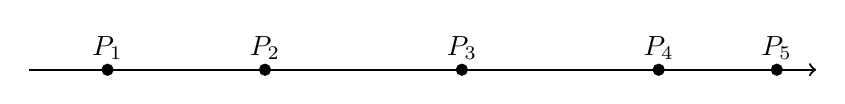
\begin{tikzpicture}[scale=1]
    % Zeichne einen waagerechten Pfeil
    \draw[->, thick] (0,0) -- (10,0);

    % Punkte P1 bis P5 in unregelmäßigen Abständen
    \filldraw (1,0) circle (2pt) node[above] {$P_1$};
    \filldraw (3,0) circle (2pt) node[above] {$P_2$};
    \filldraw (5.5,0) circle (2pt) node[above] {$P_3$};
    \filldraw (8,0) circle (2pt) node[above] {$P_4$};
    \filldraw (9.5,0) circle (2pt) node[above] {$P_5$};
\end{tikzpicture}


\textbf{Trick:} \\
Permutiere $p_1, \dots, p_n$ zufällig und hoffe, dass dadurch die Anzahl der Änderung der cp-Distanz gering bleibt.

\subsubsection{Algorithmus:}
\begin{enumerate}
    \item Bringe Punkte in zufällige Reihenfolge $p_1, \dots, p_n$
    \item $\delta_2 = |p_1 p_2|$
    \item D $\leftarrow$ Gitterstruktur mit Maschenweite $ \delta_2$ welche $\{p_1, p_2\}$ enthält
    \item 
    \begin{lstlisting}
        for i to n do
            platziere $P_i$ in D
            untersuche die 9 relevanten Gitterzellen auf potentielle CPs mit $p_i$
            if $\nexists p_j, j<i$ mit $|p_i p_j | < \delta_{i-j}$ gibt then
                tue nichts, $\delta_i = \delta_{i-1}$
            else 
                $\delta_i = min|p_jp_i|$ mit $j<i$
                D $\leftarrow$ Gitterstruktur mit Maschweite $\delta_i$, welche $\{p_1, \dots, p_i\}$ enthaelt
        od
    \end{lstlisting}
    \item return $\delta_n$
\end{enumerate}

\subsubsection{}
\textbf{Analyse:} Betrachte Einfügung von Punkt $p_i$. Es gibt zwei Fälle:
\begin{enumerate} [label=\Alph*.]
    \item (billig) $\delta_i = \delta_{i-1}$, d.h. $p_i$ erzeugt kein neues CP.
    \item (teuer) $\delta_i < \delta_{i-1}$, d.h. $p_i$ erzeugt neues CP. 
\end{enumerate}

Sei $\{p_a,p_b\} \subset \{p_1, \dots, p_i\} $ das  CP in $\{p_1, \dots, p_i\}$.\\
Die Einfügung von $p_i$ ist genau dann teuer, wenn $p_i = p_a\ oder\ p_i=p_b$.\\
\\
Da die Punkte $\{p_1, \dots, p_i\} $ zufällig gleichverteilt permutiert sind, ist diese Wahrscheinlichkeit $\leq \frac{2}{i}$.

$\implies$ Erwartete Kosten der Einfügung von $p_i$ sind:

\begin{align*}
    P_r(\text{teure Einfuegung}) \cdot O(i) + P_r(\text{billige Einfuegung}) \cdot O(1) &= O\left(\frac{1}{i}\right) \cdot O(i) + O(1) \\
    &= O(1)
\end{align*}

Gesamtkosten des Algorithmus sind die Summen der Kosten der Einfügungen $p_1,p_2, \dots, p_n$.\\
Sei $X_c $ eine ZV, welche die Kanten der Einfügung von $p_i$ benennt und X eine ZV, welche die Gesamtkosten benennt. Es gilt:

 \[X=X_1 + X_2 + \dots + X_n = \sum_{i=1}^{n}(X_i) \]
 \[ E(X) = E\left(\sum_{i=1}^{n}X_i\right) = \sum_{i=1}^{n}\underbrace{E(X_i)}_{= O(1)} = O(n) \]


\textbf{Sehr wichtig}: Die Laufzeit unseres Algorithmus ist immer erwartet O(n), egal wie die Eingabe aussieht.\\
\\
\textbf{Auch wichtig:} Algorithmus berechnet immer das korrekte Ergebnis, nur die Laufzeit. kann variieren aufgrund des Zufalls.\\

$\implies $ LAS VEGAS ALGORITHMUS\\

\subsection{MinCut-Problem}
\textbf{Gegeben:} ungerichteter, ungewichteter (Multi)-Graph G(V,E) mit $|V| = n , |E| = m$ \\
Ein Cut(Schnitt) $\phi$ von G ist definiert durch eine Partition V = $ V_1 \uplus V_2 $ der Knoten $|V_i|>0$.\\
Der Wert des Cuts $\phi$ ist:

\[ |\{ e=\{v,w\} \in E | v \in V_1, w \in V_2 \}| \]

\textbf{Ziel:} Bestimme den Cut $\phi$ mit minimalem Wert.\\
Bsp.: Bild von Graph


\subsection{Las Vegas Algorithmus: Closest Pair (bruder meinte iwo sollen Fehler in den Bezeichnern sein) }
Laufzeit von $O(n)$\\
Kann nur quadratische Zeitdauer haben wenn der Algorithmus quadratisch würfelt
{\bf Problem:} Gegeben sei eine Punktmenge $P=\{p_1, p_2, \dots, p_n\}$ im $\mathbb{R}^2$. Ziel ist es, Punkte $p,q\in P, p\neq q$ zu finden sodass $|pq|\leq |p'q'|$ für alle $p', q'\in P, p'\neq q'$.

Deterministisch können wir dieses Problem in $O(n\log n)$ lösen, z.B. mittels eines Divide\&Conquer-Algorithmus. Unter der Annahme, dass wir in konstanter Zeit hashen können, zeigen wir einen randomisiert inkrementellen Algorithmus, der das Problem in erwartet $O(n)$ Zeit löst. 
 
\begin{algorithm}
	\KwData{Point set $P$}
	\KwResult{$\min_{p,q\in P, p\neq q} |pq|$}
	randomly permute $P$ to $\{p_1, p_2, \dots, p_n\}$\;
	$\delta_2 \gets |p_1p_2|$\;
	$D\gets$ grid structure with cell width $\delta_2$, containing $p_1, p_2$\;
	\For{$i\gets 3$ \KwTo $n$}{
		put $p_i$ into $D$\;
		check $9$ relevant grid cells for new closest pair with $p_i$\;
		\If{$\nexists p_j$ with $j<i$ and $|p_jp_i|<\delta_{i-1}$}{
			$\delta_i\gets \delta_{i-1}$\;
		}
		\Else{
			$\delta_i\gets \min_{j<i} |p_jp_i|$\;
			$D\gets$ grid structure with cell width $\delta_i$, containing $p_1, \dots, p_i$\;
		}
	}
	return $\delta_n$\; 
\end{algorithm}

Zentrale Einsicht beim Beweis der Laufzeit ist folgendes Lemma:
\begin{lem}
	Die Wahrscheinlichkeit, dass bei Hinzunahme von $p_i$ die Gitterstruktur neu aufgebaut werden muss, ist $\leq 2/i$.
\end{lem}
\begin{proof}
Wir nehmen zunächst an, dass die closest pair Distanz eindeutig ist und von nur zwei Punkten definiert wird.
	Seien nun $P_i=\{p_1, p_2, \dots p_i\}$ und $p_a, p_b\in P_i$ die beiden Punkte aus $P_i$, welche das closest pair in $P_i$ definieren.
	Die Gitterstruktur muss genau dann neu aufgebaut werden, wenn $p_i=p_a$ oder $p_i=p_b$. Da die Reihenfolge jedoch zufällig gleichverteilt ist, ist jeder der ersten $i$ Punkte mit gleicher Wahrscheinlichkeit $p_i$.
	Daher ist die Wahrscheinlichkeit, dass $p_i$ entweder $p_a$ oder $p_b$ ist, genau $2/i$. Falls die closest pair Distanz von mehr als zwei Punkten definiert wird, ist die Wahrscheinlichkeit, dass die Gitterstruktur neu
	aufgebaut werden muss, nur noch geringer.
\end{proof}



\subsection{Monte Carlo Algorithmus: Karger's MinCut Algorithmus}
(Übung einfach mal integrieren) \\
{\bf Problem:} Gegeben einen ungewichteten, ungerichteten Multigraph $G(V,E)$, bestimme eine Partition $V=V_1 \mathop{\dot\cup} V_2$ der Knotenmenge mit $V_1,V_2\neq \emptyset$, sodass der induzierte Schnitt $$cut(G, V_1):=\bigl\{\{v,w\}\in E: v\in V_1, w\in V-V_1 \bigr\}$$ minimale Kardinalität hat. Der Wert des Cuts ist $= $

Bekannte Algorithmen wie Edmonds-Karp lösen dieses Problem deterministisch in Zeit $O(m^2n)$, wobei $n=|V|, m=|E|$ $e= v,w \in E$ \\
\textbf{Ziel: } Beste Knotenpartition mit minimalem Cut Wert. \\
\textbf{Determinismus:} Stoer-Wagner-Algorithmus löst das Problem in $O(nm + n^2 log n)$. \\
\textbf{Randomisierter Algorithmus: } hat Laufzeit $O(n^2 log^3$n) 
\textbf{Naive Lösung: } Alle Partitionen überprüfen, dauert aber $2^n$ lang, weil $2^n$ viele. \\
\subsection{Zentrale Operation des neuen Algortihmus}
Kantenkontraktion (nimmt die Knoten und zieht diese zusammen inklusiver der, die an dem Hängen, einfach zwei Knoten zu einem mergen, aber wenn die gleichen Knoten beide mit einem verbunden sind, hat man sogar zwei Kanten zum gleichen Knoten und nicht nur einen \textbf{!}.) \\
\subsection{Karger Min-Cut Algorithmus}

\textbf{Algorithmus: Karger MinCut Algorithmus}\\

\begin{verbatim}
    for i=1 to n-2 do
        Kontrahiere zufällige Kanten
    od
    Gebe die Partition der Knotenmenge entsprechend der beiden 
    "ueberlebenden" Kanten zurueck
\end{verbatim}
Man kann den Algorithmus so implementieren, dass ein Durchlauf O(m) kostet.\\
\\
\textbf{Jetzt} beweise, dass die Wahrscheinlichkeit einen MinCut zu finden $\geq \frac{1}{n^2}$ ist. 

\begin{lem}
    Betrachte eunen Multigraph G=(V,E) mit einem MinCut mit Wert k, dann gilt: G hat mindestens $\frac{k \cdot n}{2}$ Kanten.
\end{lem}

\subsubsection{Beweis}
Beobachtung: Jeder Knoten hat Grad $\geq k$.\\
$\implies$ Es gibt $\geq \frac{k \cdot n}{2}$ Kanten.\\
\\
\textbf{Anmerkung:} Wir konzentrieren uns im folgenden auf einen fixen MinCut: $X \uplus V - X$\\

Sei $E_i$ das Ereignis, dass im i-ten Kantenkontraktionsschritt keine MinCut kontrahiert wurde.\\
Was ist die Wahrscheinlichkeit, dass im ersten Schritt keine Kante unseres MinCuts kontrahiert wird?\\
\[\implies 1 - \underbrace{\frac{k}{m}}_{\text{Wahrscheinlichkeit eine Kante des MinCuts zu erwischen}} \geq 1 - \frac{k \cdot 2}{k \cdot n} = 1 - \frac{2}{n} \ \ \ \ \ \ \ \text{mit} \ \ \frac{k}{m} \geq \frac{k \cdot n}{2}\]

%fehlt  was

$P_r(E_1)= 1-\frac{2}{n}$\\
\\
Falls $E_1$ eingetreten ist, existieren vor dem zweiten Schritt mindestens $\frac{k(n-1)}{2}$ Kanten.\\
$\implies$ Wahrscheinlichkeit im zweiten Schritt keine Kante des MinCuts zu erwischen ist dann:

\[ P_r(\epsilon_2 | \epsilon_1) = 1- \frac{k}{m'} \geq 1 - \frac{2}{n-1}\] 

Wahrscheinlichkeit im i-ten Schritt keine Kante des MinCuts zu erwischen ist: 

\[ P_r(E_i | \bigcap_{j=1}^{i-1} E_j) \geq 1 - \frac{2}{n-i+1} \] 

$\implies$ Wahrscheinlichkeit, nur eine Kante des MinCuts kontrahiert zu haben ist:

\begin{align*}
    P_r\left(\bigcap_{i=1}^{k-2} E_i\right) &= P_r(E_1) \cdot P_r(E_2 \mid E_1) \cdot P_r(E_3 \mid E_1 \cap E_2) \cdots \\
                                            &= \prod_{i=1}^{n-2} \left(1 - \frac{2}{n-i+1}\right) \\
                                            &= \prod_{i=1}^{n-2} \frac{n-i+1-2}{n-i+1} \\
                                            &= \prod_{i=1}^{n-2} \frac{n-i-1}{n-i+1} \\
                                            &= \frac{\cancel{n-1}}{n} \cdot \frac{\cancel{n-3}}{n-1} \cdot \frac{\cancel{n-4}}{\cancel{n-2}} \cdot \frac{\cancel{n-5}}{\cancel{n-3}} \cdot \frac{\cancel{n-6}}{\cancel{n-4}} \cdot \dots \cdot \frac{2 \cdot 1}{\cancel{4 \cdot 3}} \\
                                            &= \frac{2}{n(n-1)}
\end{align*}



$\implies$ Wahrscheinlichkeit keine Kante des MinCuts zu kontrahieren ist $\geq \frac{2}{n(n-1)} \geq \frac{1}{n^2}$\\
\\
Eine Erfolgswahrscheinlichkeit von $\sim  \frac{1}{n^2}$ klingt nicht sehr überzeugend, durch Wiederholung und Bestimmung des besten Resultats der
Wiederholungen können wir die Erfolgswahrscheinlichkeit beliebig erhöhen.\\
Wenn wir den Algorithmus $\frac{n^2}{2}$ - mal wiederholen, ist die Wahrscheinlichkeit nie den echten MinCut gesehen zu haben:

\[(1- \frac{2}{n(n-1)})^{\frac{n^2}{2}} \underbrace{\leq}_{1-x \leq e^{-x}} (e^{\frac{-2}{n(n-1)}}) < \frac{1}{e} \] 

%fehlt was

Also wissen wir, dass die Wahrscheinlichkeit nach $\frac{n^2}{2}$ Wiederholungen den echten MinCut berechnet zu haben midestens $1- \frac{1}{e} \approx 0.63$
ist.\\

Durch noch mehr Wiehderholen lässt sich die ErfolgsWahrscheinlichkeit beliebig erhöhen, z.B:\\

$10 \cdot \frac{n^2}{2}$ wiederholen $\implies$ Fehlerwarscheinlichkeit $<(\frac{1}{e}^{10}) \approx 0,000045$.\\
Das geht in Laufzeit $O(m \cdot n^2)$ (Vergleiche mit $O(n \cdot m + n^2 \cdot log(n)))$ deterministisch)\\
\\
Dieser Algorithmus gehört zur Klasse der Monte-Carlo Algorithmen, deren Korrektheit hängt vom Zufall ab.\\
\\
Wenn wir z.B. $ c \cdot \frac{n^2}{2} \cdot log(n)$ wiederholbar, ist die Fehlerwarscheinlichkeit $\approx \frac{1}{n}$. ''Erfolg tritt mit hoher Wahrscheinlichkeit ein''\\
\\
Wenn wir z,B $ c \cdot \frac{n^2}{2} \cdot n$ wiederholbar, ist die Fehlerwarscheinlichkeit $\approx \frac{1}{2^n}$. ''Erfolg tritt mit sehr hoher Wahrscheinlichkeit ein''\\


\subsection{Unterschiede LasVegas und MonteCarlo Algorithmen}

\begin{table}[h]
    \centering
\begin{tabular}{c|c}

    Closest Pair & MinCut\\
    \hline
    liefert immer korrektes Resultat, egal wie sich Zufall verhält & Kann falsches Ergebnis liefern abhängig von Zufall\\
    \hline
    Laufzeit abhängig von Zufall & Laufzeit fix für gegebene Fehlerschwelle \\
    \hline
    LasVegas & MonteCarlo
    
\end{tabular}
\end{table}
Man kann aus jedem Las Vegas Algorithmus einen Monte Carlo Algorithmus machen. Sei f(n) die erwartete Laufzeit des Monte Carlo Algorithmus,
wir lassen den Algorithmus für $ \alpha \cdot f(n)$ mit  $\alpha > 1$. Falls Alg. bis dahin terminiert:\\
$\implies$ Ergebnis korrekt, sonst brechen wir ab und geben irgendwas aus.\\
\\
Dieser modisierte Alg. hat Laufzeit. von $\alpha \cdot f(n)$.\\
$\implies$ müssen noch ErfolgsWahrscheinlichkeit berechnen\\
\\
\textbf{Markov-Ungleichung}\\
Sei X eine nicht negative ZV mit $E(X) = \mu$, Dann gilt: $P_r (X> \alpha \cdot \mu) \leq \frac{^1}{\alpha}$\\
$\implies$ Unser modifizierter, abbrechender LV Algorithmus hat Fehlerwarscheinlichkeit $\leq \frac{1}{\alpha}$.\\
\\
MC $\rightarrow$ LV machbar?\\
Falls wir neben dem MC Algorithmus mit Laufzeit f(n) und ErfolgsWahrscheinlichkeit p(n) einen Checker-Algorithmus C mit Laufzeit g(n) haben, der
Korrektheit überprüfen kann, machen wir folgendes:

\begin{enumerate}
    \item lasse MC Algorithmus laufen
    \item checke ob korrekt, falls nein gehe zu 1.
\end{enumerate}

Pro Runde ist Laufzeit. $f(m)+g(n)$\\
Die erwartete Anzahl Runden bis zum Erfolg $\frac{1}{p(n)} \implies$ erwartete Laufzeit. $\frac{f(n)+g(n)}{p(n)}$.

\subsection{Monte Carlo Algorithmus: Karger's MinCut Algorithmus}
{\bf Problem:} Gegeben einen ungewichteten, ungerichteten Multigraph $G(V,E)$, bestimme eine Partition $V=V_1 \mathop{\dot\cup} V_2$ der Knotenmenge mit $V_1,V_2\neq \emptyset$, sodass der induzierte Schnitt $$cut(G, V_1):=\bigl\{\{v,w\}\in E: v\in V_1, w\in V-V_1 \bigr\}$$ minimale Kardinalität hat.

Der deterministische Stoer-Wagner Algorithmus löst das Problem (für gewichtete Graphen) in $O(nm+  n^2\log n)$, das Problem des minimalen $s-t$-cuts wird z.B. vom Edmonds-Karp-Algorithmus in in Zeit $O(m^2n)$ gelöst, wobei $n=|V|, m=|E|$. Wir betrachten im Folgenden einen randomisierten Monte-Carlo-Algorithmus für dieses Problem mit (verbesserter) Laufzeit $O(n^2 \log^3 n)$, der den MinCut mit Wahrscheinlichkeit $\Omega(1-1/n)$ bestimmt.

Zentrale Operation des Algorithmus ist die Kontraktion zweier adjazenter Knoten. Hierbei werden alle bestehenden Kanten übernommen, Schleifen jedoch gelöscht. Der Algorithmus selbst ist dann sehr simpel, es wird in $n-2$ Runden jeweils eine zufällige Kante ausgewählt und die entsprechenden Knoten kontrahiert.

\begin{algorithm}
	\For{$i\gets 1$ \KwTo $n-2$}{
		select a random edge $\{v,w\}$ and contract nodes $v$ and $w$
	}
	return vertex sets corresponding to two surviving nodes
\end{algorithm}

Fixieren wir einen konkreten MinCut, so wird dieser genau dann gefunden, wenn während des Ablaufs des Algorithmus, nie eine Kante dieses MinCuts kontrahiert wird. Wir wollen im Folgenden eine untere Schranke dafür beweisen, dass ein konkreter MinCut gefunden wird.

\begin{lem}
	Betrachte einen Multigraph $G(V,E)$, der einen MinCut mit Wert $k$ enthält. Dann gilt: $G$ hat mindestens $\frac{kn}{2}$ Kanten.

\end{lem}

\begin{lem}
	Sei $(X,V-X)$ ein fixer MinCut. Unter der Annahme, dass in den $i-1$ vorherigen Kontraktionen keine Kante diese MinCuts kontrahiert wurde, ist die Wahrscheinlichkeit, bei der $i$-ten Kontraktion keine Kante dieses MinCuts zu kontrahieren mindestens $1-\frac{2}{n-i+1}=\frac{n-i-1}{n-i+1}$. 
\end{lem}

\begin{lem}
	Die Wahrscheinlichkeit, dass obiger Algorithmus einen fixen MinCut findet ist mindestens $\frac{2}{n(n-1)}$
\end{lem}

Dadurch, dass wir den Algorithmus $n^2/2$ oft wiederholen und den Cut mit kleinstem Gewicht zurück geben, können wir die Erfolgswahrscheinlichkeit deutlich erhöhen:

\begin{lem}
	Bei $n^2/2$ Wiederholungen ist die Wahrscheinlichkeit, einen fixen MinCut zu finden mindestens $1-1/e$.
\end{lem}

Durch weitere Wiederholungen lässt sich die Erfolgswahrscheinlichkeit beliebig verbessern, so führen z.B. $c\cdot \log n  \cdot \frac{n^2}{2}$ Wiederholungen zu einer Erfolgswahrscheinlichkeit von mindestens $1-\frac{1}{n^c}$

\subsubsection{Verbesserung der Erfolgswahrscheinlichkeit (Karger-Stein)}
Die Erfolgswahrscheinlichkeit des ursprünglichen Karger-MinCut Algorithmus kann deutlich verbessert werden, indem man eher späte Kontraktionen mehrfach/oft wiederholt(anstatt alle oft zu wiederholen), da gerade diese eine größere Wahrscheinlichkeit haben, eine MinCut-Kante zu kontrahieren. Zunächst beobachten wir, dass es recht wahrscheinlich ist, in den ersten $n-n/\sqrt{2}-1$ Kontraktionsschritten keinen Fehler zu machen:

\begin{lem}
	Die Wahrscheinlichkeit, dass man von einem fixen MinCut bei  $n- \frac{n}{\sqrt{2} }-1$ Kontraktionsschritten eine Kante dieses MinCuts kontrahiert, ist $\leq 1/2$.
\end{lem}
\begin{proof}
	Wie in der Grundversion des Karger Algorithmus ist die Wahrscheinlichkeit, diesen MinCut in der $i$-ten Kontraktion nicht zu zerstören (unter der Annahme ihn davor schon nicht zerstört zu haben) mindestens $1-\frac{2}{n-i+1}=\frac{n-i-1}{n-i+1}$. Die Wahrscheinlichkeit, ihn in den ersten $i$ Kontraktionsschritten nicht zu zerstören (also basically Erfolgswahrscheinlichkeit) ist somit $\frac{(n-i-1)(n-i)}{n(n-1)}$.
	Für $i=n-n/\sqrt{2}-1$ ergibt sich somit $\frac{(n/\sqrt{2})(n/\sqrt{2}+1)}{n(n-1)}=\frac{n^2/2+n/\sqrt{2}}{n(n-1)}=\frac{n/2+1/\sqrt{2}}{(n-1)}=\frac{1}{2}\frac{n+\sqrt{2}}{n-1}\geq \frac{1}{2}$
\end{proof}

Wir nutzen dies dann in folgender Variation des Algorithmus:
\begin{algorithm}
	\SetKwProg{Fn}{Function}{is}{end}
	\Fn{KargerStein(G)}{
		$G_1' \gets$ graph after $n- \frac{n}{\sqrt{2} }-1$ random contractions\;
		$G_2' \gets$ graph after $n- \frac{n}{\sqrt{2} }-1 $random contractions\;
		$(C_1, V-C_1)=KargerStein(G_1')$\;
		$(C_2, V-C_2)=KargerStein(G_2')$\;
		return smaller of the two cuts
	}
	
\end{algorithm}

Sei $T(n)$ die Laufzeit dieses Algorithmus für einen Graph mit $|V|=n$. Exklusive der Rekursion, verbraucht ein Aufruf $O(n^2)$ Zeit für die Kontraktionen. Somit haben wir $T(n)=O(n^2)+ 2T(n/\sqrt{2})$ (weil Rekursion).
\begin{lem}
	Es gilt $T(n)=O(n^2 \log n)$.
\end{lem}
Interessant ist nun die Analyse der Wahrscheinlichkeit $P(n)$, dass der Algorithmus einen MinCut berechnet.
\begin{lem}
	Es gilt $P(n)\geq 1/\log n$.
\end{lem}
\begin{proof}

	Wir beweisen per Induktion und nehmen an, es gelte $P(i)\geq 1/\log i$ für $i<n$. Mit Wahrscheinlichkeit $\frac{1}{2}\cdot P(n/\sqrt{2})$  (das ist so, weil man bei der Konstruktion von $ G_1 ´$ keinen Fehler gemacht haben muss und die Rekursion zurückkommen muss und dafür hat man ja schon das p definiert) ist $(C_i, V-C_i)$ ein MinCut, d.h. kein MinCut wird gefunden mit der entsprechenden Gegenwahrscheinlichkeit:
	\[
		P(n)\geq 1- (1- \frac{1}{2}P(n/\sqrt{2}))^2 \geq  1-(1-\frac{1}{2\cdot (\log n - 1/2)}))^2= 1- (1-\frac{1}{2\log n -1})^2 
	\]
	\[
		=1 - 1 + \frac{2}{2\log n -1} - \frac{1}{(2\log n -1)^2}
	\]
	\[
		=\frac{1}{\log n -1/2} - \frac{1}{(2\log n -1)^2} =\frac{\log n }{\log n(\log n -1/2)} - \frac{1}{(2\log n -1)^2} 
	\]
	\[
		=\frac{\log n +1/2 - 1/2}{\log n(\log n -1/2)} - \frac{1}{(2\log n -1)^2} 
	\]
	\[
		=\frac{1}{\log n} + \frac{1/2}{\log n(\log n -1/2)} - \frac{1}{(2\log n -1)^2} 
	\]
	\[
		=\frac{1}{\log n} + \frac{1}{\log n(2\log n -1)} - \frac{1}{(2\log n -1)^2} 
	\]
	\[
		=\frac{1}{\log n} + \frac{2\log n -1-\log n}{\log n(2\log n -1)^2} 
	\]
	\[
		\geq =\frac{1}{\log n} 
	\]
\end{proof}

Nun reichen wenige Wiederholungen dieses Algorithmus, um eine recht hohe Erfolgswahrscheinlichkeit zu erreichen:

\begin{lem}
	Wiederholen wir KargerStein $\log n$ mal,  erreichen wir eine Erfolgswahrscheinlichkeit von $1-1/e$. 
\end{lem}
\begin{proof}
	Die Wahrscheinlichkeit nach $(\log n)$ Wiederholungen keinen MinCut gefunden zu haben ist
	\[
		\leq (1-\frac{1}{\log n})^{\log n}\leq e^{-\frac{\log n}{\log n}}=\frac{1}{e}
	\]
\end{proof}
\textit{Vorher zum Vergleich: }
Man vergleiche das mit den $\approx n^2$ Wiederholungen, die der ursprüngliche Karger Algorithmus zur Erreichung derselben Erfolgswahrscheinlichkeit benötigt hatte. also $O(n^2 log^2 n)$ vs $O(n^4)$

\subsection{Monte Carlo Algorithmus: Verifikation von Matrix Multiplikation(Freivalds)}
Gegeben $A,B,C \in \mathbb{R}^{n\times n}$ möchten wir wissen, ob $A\cdot B=C$. Naiv geht dies in $O(n^3)$ durch Berechnung von $AB$ und Vergleich mit $C$, alternativ könnte man z.B. Strassens Algorithmus (ca. $O(n^{2.81})$ anwenden.
Also naiv: ausrechnen und verifizieren.
Folgender Monte-Carlo-Algorithmus verifiziert in $O(n^2)$ mit einer konstanten \textit{ einseitigen}(wenn er nein sagt stimmt es immer, aber wenn er ja sagt, kann es auch falsch sein) Fehlerwahrscheinlichkeit (Freivalds):
\begin{algorithm}
	choose $r\in \{0,1\}^n$ u.a.r.\;
	check whether $A\cdot (B \cdot r)=C\cdot r$\;
\end{algorithm}
Beides auf jeder Seite läuft in $O(n^2)$ 
Der Algorithmus läuft offensichtlich in $O(n^2)$ Zeit. Falls der Algorithmus Ungleichheit feststellt, gilt offensichtlich $AB\neq C$. Es bleibt zu zeigen, dass die Wahrscheinlichkeit, dass die Wahrscheinlichkeit, eine  Ungleichheit zu entdecken, groß genug ist. 

\begin{lem}
	Falls $AB\neq C$ gilt: $P(A(Br)=Cr)\leq 1/2$. P steht für Wahrscheinlichkeit.
\end{lem}
\begin{proof}
	Sei $D=AB-C$. Es gilt $ABr=Cr \Leftrightarrow (AB-C)r=0  \Leftrightarrow Dr=0$.
	Wir wissen, dass $D$ nicht die Nullmatrix ist,  sei o.B.d.A. $d_{11}\neq 0$. Es muss gelten 
	\[
		\sum_{j=1}^{n} d_{1j} r_j =0
	\]
	aufgelöst nach $r_1$ erhält man
	\[
		r_1=\frac{-\sum_{j=2}^{n} d_{1j}r_j}{d_{11}}
	\]
	Für fixe $r_2, \dots r_n$ gibt es nur einen Wert für $r_1$, der die Gleichung erfüllt. Das heißt mit Wahrscheinlichkeit $\geq 1/2$ wird ein Fehler entdeckt.
    Dh wenn wir $r_2,...., r_n$ schon zufällig bestimmt haben gibt es für $r_1$ genau eine Wahl, die $A\cdot (B\cdot r) = C \cdot r$ mal , $r_1$ ist aber nur Wahrscheinlichkeit $\frac{1}{2}$ die restliche Wahl.
\end{proof}
\subsection{Las Vegas Algorithm: QuickSort }
\begin{verbatim}
    a[1,...,n]
    wähle Pivot p in {1,...,n}
    rearrange A sodass
    <= A[p] | A[p] | > A[p]
    QS(A_left)
    QS(A_right)
\end{verbatim}
Idealerwesie hat man p so, dasss $|A_l|, |A_r| \leq \frac{h}{2} $ also p als Median gewählt.\\
Berechnet es in Linearzeit aber praktisch relativ teuer. \\
Wir wollen prakatisch teure Bestimmung des Medians vermeiden $\Rightarrow$ wähle p zufällig gleichverteilt in ${1,...,n}$ \\
\textbf{Laufzeitanalyse: }\\
Bennene die zu sortierenden Elemente $s_1,..., s_n$ gemäß der natürlichen Ordnung also $s_1 < s_2.... < s_n$ \\
Definiere ZV $X_i,j =: $ 1 falls $s_i $ mit $s_j$ verglichen wurde, 0 sonst \\
Uns interessiert 
\[
\sum_{i<j} X_{i,j}:= X( Anzahl Vegleiche) 
 \]
 Was ist E(X)\\
 basically
 \[
  \sum_{i,j} Pr(X_{i,j} =1)
 \]
 
\begin{lem}
	Die erwartete Laufzeit des randomisierten QuickSort Algorithmus ist $O(n\log n)$
\end{lem}
\begin{proof}
\end{proof}
Uns interessiert im Folgenden $Pr(X{i,j} =1)$
Stelle den Ablauf von QuickSort als Rekursionsbaum dar und schreibe jeweils das PivotElement in den entsprechenden Knoten.
\begin{figure}
    \centering
    \includegraphics[width=0.25\linewidth]{requwgdl.png}
    \caption{Hässliche Veranschaulichung}
    \label{fig:enter-label}
\end{figure}
Wir bennenen die Pivotelemente von oben nach unten/links nach rechts  \\
\Rightarrow wir bekommen Permutation $\pi = s_7 s_3 s:20 \dots$ \\
Wir suchen $\pi $ aus, wenn $s_i$ nicht mit $s_j$ verglichen wird? \\
Dann taucht ein Element $s_k $ mit $i<k<j $ als Pivotelement vor $s_i & s_j$ in $\pi$ auf. \\
$si_i$ wird mit $s_j$ genau dann verglichen, wenn $s_i$ oder $s_j$ das erste Element aus $ Mengenklamern{s_i, s_{i+1}, ...., s_j}$ \\
Mit gleicher Wahrscheinlichkeit ist jedes der $s_i,....s_j$ das erste Elementm das i -$\pi$ auftaucht.  \\
\Rightarrow $Pr( s_i$ mit $s_j$ verglichen= $\frac{2}{j-i+1}$ \\
$Pr( X_{i,j} =1$ \\
Einstöpseln:\\
$E(X) = \sum_{i<j} Pr( X_{i,j} = 1$ = $ \sum_{i<j} \frac{2}{j-i+1}$ \\
= $\sum_{i=1} ^{n-1} \sum \frac{2}{j-i+1}= $ $\sum_{i=1} ^{n-1} noch ein sum  \frac{2}{j}$
Dann iwie Integral $\frac{1}{i}$ \\
basicall $O(n logn) $ \\
\subsubsection{Exkurs: Median in deterministisch $O(n)$ Zeit /\textit{k select}}
Wir betrachten im Folgenden das Problem, das $k$-t größte Element eines Arrays $A[]$ zu bestimmen; das ist noch allgemeiner als die Bestimmung des Medians, da wir einfach $k=n/2$ setzen können.
\begin{algorithm}
	\SetKwProg{Fn}{Function}{is}{end}
	\Fn{kSelect(A[1\dots n],$k$)}{
		build $\lceil n/5\rceil$ groups of $5$ elements each \;
		for each group $i$, determine its median $m_i$, $i=1, \dots \lceil n/5 \rceil$ \;
		set $M=\{m_i:  i=1, \dots  \lceil n/5 \rceil \}$ \;
		$\widetilde{m}=$kSelect($M$, $|M|/2$)\;
		Partition $A$ into $A_L$, $\widetilde{m}$, $A_R$ \;
		\If{$|A_L|=k-1$}{
			return $\widetilde{m}$\;
		}
		\ElseIf{$|A_L|\geq  k$}{
			return kSelect($A_L$, $k$)\;
		}
		\Else{
			return kSelect($A_R$, $k-|A_L| -1$)\;
		}
	}
\end{algorithm}
Behauptung: 
\[
|A_L||A_R| \leq \frac{7}{10}n 
\}
$\widetilde{m}$  war Median der Mediane der 5er Gruppe \\
$\Rightarrow$ in jeder dieser Gruppen waren 2 Elemente echt kleiner als $m_i$, d.h. es gibt mindestens 
\[
\frac{n}{10} + \frac{2}{10}n
\]Elemente kleiner $\widetilde{m}$. \\
$\Rightarrow$ mindestens $\frac{3}{10} n$ Elemente sind kleiner als $\widetilde{m}$. \\
$\implies$ 
\[
|A_L| , |A_L| \leq \frac{7}{10}
\]
\[
T(n)= O(n) +  T(\frac{n}{5})+ T(\frac{7}{10}n)
\]
\begin{figure}
    \centering
    \includegraphics[width=0.5\linewidth]{qerzwggjdlökjbhdka.png}
    \caption{Rekursiver Baum}
    \label{fig:enter-label}
\end{figure}
\[
also \frac{9}{10} dann \frac{81}{100}n = (\binom{9}{10}^2 
\]
\[
T(n) = O(n) = \sum_{i=1} (\frac{9}{10})^i  = 10
\]
\begin{lem}
	DSelect berechnet das $k$-t größte Element eines Arrays in $O(n)$.
\end{lem}
\begin{proof}
\end{proof}
KSelecte deterministisch relativ kompliziert und praktisch nicht gut. Randomisierte Version viel besser:
\subsection{Las Vegas Algorithm: QuickSelect}
\begin{algorithm}
	\SetKwProg{Fn}{Function}{is}{end}
	\Fn{RandSelect(A[1\dots n],$k$)}{
		pick $i\in \{1, \dots, n\}$ u.a.r. \;
		partition $A$ into $A_L$, $A[i]$, $A_R$ \;
		\If{$|A_L|=k-1$}{
			return $A[i]$\;
		}
		\ElseIf{$|A_L|\geq  k$}{
			return RandSelect($A_L$, $k$)\;
		}
		\Else{
			return RandSelect($A_R$, $k-|A_L|$)\;
		}
	}
	
\end{algorithm}
Seien wir zudem pessimsitisch, dass wir immer die größere Hälfte der Rekursion ausführen müssen. \\
\[
T(n) = n + \frac{1}{n} \sum_{i=0} T(max(i,n-i+1))
\]
\[
= n + \sum_{i = \lfloor \frac{n}{2}\rfloor } T(i)
\]
\begin{proof}
Wollen per Induktion zeigen: $T(n) \leq c \cdot n$ \\

\[
n-1 \rightarrow n: T(n) = n + \frac{2}{n} \sum_{i= \frac{n}{2}\rfloor} c \cdot i
\]
\[
= n + \frac{2c}{n} \sum_{i = \lfloor \frac{n}{2}\rfloor }
\]
\[
\leq n + \frac{3}{4}c)
\]
\[
\leq \frac{3}{8} n^2 = n(1+ \frac{3}{4}c) 
\] ok für 
\[
1+ \frac{3}{4}c 
\]
\[\leq c
\]
Also praktisch ist also randomisiert einfacher da determibistisch aufwendiger ist.
\end{proof}

\begin{lem}
	RandSelect berechnet das $k$-t größte Element eines Arrays in erwartet $O(n)$.
\end{lem}
\begin{proof}
\end{proof}



\subsection{Hashing}
Ein Wörterbuch besteht aus einer  Menge von Items, welche jeweils aus einem \textit{Schlüssel} und assoziierten \textit{Informationen} besteht.\\ 
\newline
Jedes Item wird eindeutig  durch seine Schlüssel identifiziert.
\textit{Beispiel}
\begin{itemize}
    \item Stowasser \\
    \textit{Schüssel:} Lat. Wort. \\
    Information: Übersetzung/Erklärung des Wortes
    \item Telefonbuch \\
    \textit{Schlüssel: } Name + Vorname \\
    \textit{Information:} Telefobuch/Adresse 
    \item Im randomisierten Closest  Pair Algorithmus: \\
    \textit{Schlüssel: } Gitterzahlkoordinaten \\
    \textit{Information: } Menge der unlesbar in dieser Zelle
\end{itemize}
Wenn wir ein Wörterbuch als abstakte Datenstruktur  auffassen, hätten wir gerne u.a folgende Operationen darauf: 
\begin{verbatim}
   S.insert(x)... fügt Item x in S  ein
   S.delete(x) ... löscht item x aus S
   s-lookup(k)...findet item k welches Schlüssel k hat.
\end{verbatim}
\subsubsection{Naivies Implementieren}
\begin{enumerate}
    \item Lege Vektor an für Items samt Zähler für Anzahl an Items in S \\
    S.lookup(k)... alle Items durchgehen \\
    s.delete(x) .... item finden, löschen, letztes Element an freie Stelle kopieren und Zähler runtersetzen \\
    s.insert(k) ... Item x hinten anhängen, Zähler erhöhen.(nach Test, ob x nicht schon in S ist) \\
   $\Rightarrow$ alle in $O(n)$  (item ist echt das Paar aus Schlüssel und info)
   \item Ähnlich,  aber mittels verketteter Liste $\Rightarrow$ auch nicht gut aber
   \item ALternativ:  verwalte Schlüssel in einem Suchbaum(RotSchwarz, AVL, 2,3,4- Baum) $\Rightarrow O(log n)$  für lookup, insert, delete im \textbf{worst case}
   \item \textit{Direkte Addressierung: } \\
   Annahme: Schlüsseluniversum ist $ [0,...N-1]$ \\
   Speichere Arrays in Größe $N$. \\
   An Stelle i steht das Item mit Schlüssel(i), falls vorhanden, \\
   $\Rightarrow$  insert/lookup/delete alles in $O(n)$. \\
   Dass das Problem Platzverbrauch ist und der ungefähr  die Größe des Schlüsseluniversums ist, überrascht nur Opfer.
\end{enumerate}
\begin{defi}[Hashing]
	Gegeben sei ein Universum $U=\{0, \dots, N-1\}$, eine abzuspeichernde Schlüsselmenge $S\subset U$, $|S|=n$ sowie eine Hashtafel $T$ der Größe $t$.
    
	Ziel ist die Bestimmung einer Hashfunktion 
    \[
    h: U\rightarrow \{0, \dots, t-1\}\]
    , sodass
    \[
    c_x(S)\leq \lceil \frac{|S|}{t}\rceil
    \]
    für alle $x\in S$.   \\Hierbei sei 
    \[
    c_x(S):=|\{y\in S: h(y)=h(x)\}|
    \]
\end{defi}
Also Nummern der Schubladen blyat.
S  ist eine Teilmenge also das Schlüsseluniversum wären wirklich alle möglichen Lösungen an Vor und Nachnamen. \\
\newline
Intuitiv wollen wir, dass die gesuchte Hashfunktion $h$ die Schlüsselmenge $S$ 'gleichmäßig' über die Hashtafel verteilt.

\subsubsection{Beispiel: }
$U=N$ \\
$S={20,13,6,18.28,31}$ \\
$t= 5$ \\
$h(x)= x mod5$ \\
Für $S= {11,33,22,19,5}$  ist diese Hashfunktion perfekt
\begin{figure}
    \centering
    \includegraphics[width=0.5\linewidth]{beispielhashTabelle.png}
    \caption{Beispiel Hashtabelle lel}
    \label{fig:enter-label}
\end{figure}
\subsubsection{Hashing mit  Verkettung}
Jede  Schublade/hashttafelposition ist Kopf einer linearen Liste. Alle $x\in S$ mit $h(x)0i$ in der i-ten Liste gespeichert. \\
Platzbedarf einer solchen Datenstruktur ist 
\[
O(t+n) = O(n(\frac{t}{n}+1)) , \beta= \frac{n}{t}
\]
Belegungsfaktor der Hashtafel. Evtl statt n k nehmen. \\
Unter der  Annahme, dass h(x) in $O(1)$ berechnet werden kann, haben wir folgende Zugriffszeiten: \\
Zugriff  auf  $x \notin S$ : $O(1+$ Länge der Liste $L_{h(x) }$) \\
Zugriff  auf  $ x \in S:$ $O(1+ $ Position von x in $L_{h(x)}$ )\\
\newline
\textbf{Annahme: } h verteilt $U$ gleichmäßig über T, dh $ \forall i: | x \in U: h(x) =i | \leq \frac{N}{t} $ (bsp h(x)= x mod t 
\subsubsection{Frage}
Gibt es eine Superfunktion h welche für jedes $S \subset U$ erreicht, dass $\forall i \in {0,...,t-1}$ $| x\in S : h(x) i \leq \frac{|S|}{t}$ ?
\begin{proof}
    Sei 
    \[
    c_x(S) = y\in S | h(y) = h(x)
    \]
    (Menge der Schlüssel  aus S, die in derselben Schublade wie x landen. \\
    \[
    c_{max}(S)= max(c_x (S)), x \in S
    \]
\end{proof}
 \begin{thm}
 Seien $U, t, h$  gegeben, $|U|=k$. Dann gibt es für alle 
n mit
\[
1\leq n\leq  \frac{k}{t} 
\]ein 
\[
S\subset U mit |S|=n
\],  mit 
\[
c_{\max}(S)=n.
\]
 Hierbei ist
\[
 c_{\max}(S)=\max_{x\in S} c_x(S)
\]
Dh alle Elemente $x \in S$ werden in der seleben Schublade gehasht. Es gibt also immer eine Hashfunktion die völlig nutzlos ist, da sie alles in die  gleiche reinhaut.
\end{thm}
\begin{proof}
Nach Schubfachprinzip  existiert  ein $0 \leq i \leq t $ sodass $|h ^{-1} (i)| $ (das ist die Menge der 
\[
x \in U: h(x)=i)>= \frac{|U|}{t} = \frac{k}{t}
\]
Da $\frac{k}{t} >= n$, wöhle einfach S  aus  $h^{-1}(i).$
\end{proof}

Die Aussage des Theorems ist, dass es keine ''Superhashfunktion'' gibt, die für alle möglichen Schlüsselmengen $S$ gut ist.


\begin{defi}[Belegungsfaktor]
	Bei Hashing mit Verkettung ist $\beta=\frac{n}{t}$ (durchschnittliche Anzahl an Elementen aus $S$ pro Hashtafeleintrag) der sogenannte Belegungsfaktor.
\end{defi}

Unter der Annahme, dass wir eine Hashfunktion $h$ haben, die $U$ (nicht $S$!) gleichmäßig über die Hashtafel verteilt, d.h. 
\[
\forall i: |\{x\in U: h(x)=i\}|\leq \lceil\frac{N}{t}\rceil
\], können wir einige Aussagen über die erwartete Zugriffszeit für zufällige Elemente treffen.

\begin{lem}
	Sei $x\in U-S$ zufällig und $n\leq N/2$. Dann ist die erwartete Suchzeit nach $x$ in $O(1+\beta)$. $\beta =$ Belegungsfaktor
\end{lem}
\begin{proof}
Sei $i=$ # Elemte aus S, die in $L_i$ gespeichert werden.
\[
\sum_{i=0} ^{t-1} l_i = n \\
\]
Die erwartete  Suchzeit x ist 
\[
\sum_{i=0} ^{t-1} l_i \cdot Pr(h(x)=i)) +1 
\]
Pr ist die Wahrscheinlcihekit, dass das actually Eintritt, also Ergebnis der Klammer \\

\[
Pr( h(x)=i = \frac{\frac{U_}{S}}{\frac{U}{S}} 
\]
\[
\leq \frac{U_i}{\frac{U}{S}} 
\]
\[
\leq\frac{N/t}{N/2}
\]
\[
\leq \frac{2}{t}+ \frac{1}{n}$ 
\]
\[
= 1+ \frac{2}{t} \sum_{i=0}^{t-1} l_i+ \frac{1}{n}\sum_{i=0}^{t-1}
\]
\[
 =1+ \frac{2n}{t}+ 1
\]
\[
 = 2+ 2\frac{n}{t}= O(1+ \beta) 
\]
\end{proof}
\textbf{Problem: } in der Praxis  sind Zugriffe in der Regel alles andere als zufällig gleichverteilt.
Im Folgenden sei $l_i=|\{x\in S: h(x)=i\}|$
\begin{lem}
	Sei $x\in S$ zufällig (gleichverteilt). Dann ist die erwartete Zugriffszeit für $x$ in 
    \[
    O(1+ \frac{1}{n}\sum_{i=0}^{t-1} \frac{l_i(l_i+1)}{2}).
    \]
\end{lem}
\textbf{Anmerkung: } die Aussage ist ziehmlich schwach, da wir wenig über 
\[
\sum_{i=0}^{t-1} \frac{l_i(l_i+1)}{2})\]
wissen, auch wenn $\summ l_i = n$. \textbf{Schwache Aussage alert.}
\begin{proof}
Wenn x das j-te Element m seiner liste ist, ist die Suchzeit $O(1+j)$ Also ist die erwartete Suchzeit \[
\[
 O(\frac{1}{n} \sum_{j=0} \sum_{j=1} ^{l_i} (1+j]] = 
\]
\[
O(\frac{1}{n} \sum_{i=0}^{t-1} \frac{l_i (l_i +1)}{2}
\]
\end{proof}

Die Aussage dieses Lemmas ist jedoch äußerst schwach, da aus 
\[
\sum l_i =
\] nichts interessantes für 
\[
\sum l_i^2
\]
folgt.  \\
Unter der Annahme, dass $S$ eine zufällige Teilmenge  aus $U$ ist, kann auch noch folgende Aussage bewiesen werden:

\begin{lem}
	Für $S\in$ $U \choose n$ zufällig, ist die erwartete Zugriffszeit auf ein $x\in S$ in $O(1+\frac{3}{2}\beta\cdot e^\beta)$.
\end{lem}

Unter zufälligem $S$ kann somit bei  sinnvoller Wahl des Belegungsfaktors eine erwartet konstante Anfragezeit erreicht werden.

Allerdings sind Anfragen in der Praxis selten wirklich zufällig. \\
\textbf{Plan: } ersetze die Annahme, dass $S\subset U$ zufällig durch zufällige  Wahl der Hashfunktion.


\subsubsection{Perfektes Hashing}
Im Folgenden möchten wir ein Schema entwickeln, welches für eine gegebene Schlüsselmenge $S$ konstante Zugriffszeit garantiert. Dazu führen wir zunächst die $c$-Universalität einer Familie von Hashfunktionen ein.
\subsection{Universelles Hashing}
Sei $X$ eine Menge  von Funktionen von $U$ nach {0,...,t-1}. 
\textbf{Definition: } Für  $c> 1 $ heißt $X$ \textbf{c-universell}, falls für alle $x,y \in U, x \neq y$ gilt: 
\[
\frac{|h \in X: h(x) =h(y) |}  {|X|} \leq \frac{c}{t}
\]
Intuitiv bedeutet das, dass der Anteil an Hashfunktionen in $\mathcal{H}$, die zwei Elemente $x,y$ auf denselben Eintrag hashen relativ gering ist, d.h. eine zufällig gewählte Hashfunktion aus $\mathcal{H}$ hasht mit recht großer Wahrscheinlichkeit $x$ in einen anderen Eintrag  als $y$.

\begin{thm}
	Für $a,b \in [0, \dots, N-1]$ sei $h_{a,b}: x\mapsto ((ax+b) \mod N) \mod t$ und sei $N$ eine Primzahl. Dann ist die Klasse $\mathcal{H}=\{h_{a,b}: 0\leq a,b\leq N-1\}$ $c$-universell mit $c=\frac{\lceil N/m\rceil}{N/m}\approx 1$.
\end{thm}
\begin{lem}
Benutzt man Hashing mit Verkettung und wählt $h \in \mathcal{H}$ zufällig aus einer $c$-universellen Hashfamilie, dann ist die erwartete Zugriffszeit:

\[
O(1 + c \cdot B)
\]

für \textit{beliebige} Mengen $S \subset U$ mit $|S| = n$, wobei der Belegungsfaktor $B = \frac{n}{t}$ ist.
\end{lem}

\begin{proof}
Die Zugriffszeit auf ein Element $x$ besteht aus zwei Teilen:
\begin{enumerate}
    \item \textbf{Berechnung der Hashfunktion}: Dies dauert konstant $O(1)$.
    \item \textbf{Durchsuchen der verketteten Liste} in der Bucket-Position $h(x)$. Die Anzahl der Elemente $y \in S$, die mit $x$ kollidieren (d.h. $h(y) = h(x)$), ist eine obere Schranke für die Zugriffszeit.
\end{enumerate}

Definiere die Indikatorfunktion:

\[
\delta_h (x,y) =
\begin{cases}
1, & \text{falls } h(x) = h(y), \\
0, & \text{sonst}.
\end{cases}
\]

Dann interessiert uns der Erwartungswert:

\[
\mathbb{E}[\text{Anzahl der Kollisionen mit } x] = \sum_{y \in S} \mathbb{E}[\delta_h(x,y)].
\]

Da $h$ zufällig aus einer $c$-universellen Familie gewählt ist, gilt für $x \neq y$:

\[
\mathbb{E}[\delta_h(x,y)] \leq \frac{c}{t}.
\]

Summiere über alle $y \in S$:

\[
\sum_{y \in S} \mathbb{E}[\delta_h(x,y)] = 1 + \sum_{\substack{y \in S \\ y \neq x}} \mathbb{E}[\delta_h(x,y)]
\]

\[
= 1 + (n-1) \cdot \frac{c}{t}.
\]

Da der Belegungsfaktor $B = \frac{n}{t}$ ist:

\[
\mathbb{E}[\text{Zugriffszeit}] = 1 + c \cdot B.
\]

Also folgt:

\[
O(1 + c \cdot B).
\]

\textbf{Sonderfall für $x \notin S$:}  
Falls $x \notin S$, ist die erwartete Anzahl an Elementen in seinem Bucket:

\[
\sum_{y \in S} \frac{c}{t} = c \cdot B.
\]

Damit bleibt die erwartete Suchzeit ebenfalls in $O(1 + cB)$.
\end{proof}

\textbf{ABER: } Zugriff ist nur \textbf{erwartet} $O(1)$, wir hätten gerne worst case $O(1)$. \\
$\Rightarrow$ zweistufiges, perfektes Matching \\
\textbf{Ideal: } Möchte h finden mit
\[
h(x) \neq h(y)  \forall x,y \in S
\]
\textbf{1.Versuch: } Einstufiges, perfektes Hashing \\
\[
|c_s(h)= (x,y) \in \binom{s}{2}: h(x) = h(y) | 
\]
Also die Anzahl an Kollisionen für S unter h. \\
\[
c_s(h) = 0 \Leftrightarrow h|_s injektiv \\
\]

\textbf{Satz: } Für zufällige h $\in \chi$ (c universell) gilt 
\[
E (c_s(h) \leq \frac{c}{t}
\]
\begin{proof}
\[
E(c_s(h))= \sum_{(x,y) \in \binom{S}{2}}E(\delta_n(x,y)) \leq\binom{n}{2} \cdot \frac{c}{t} 
\]
    \\
    ($ \frac{c}{t}$ wegen c-universell ) \\
    \end{proof}
\textbf{Korollar: } Für $t > c \cdot \binom{n}{2}$ gibt es ein h $\in \chi$ mit $h|_s$ injektiv. Also wir zeigen das für ein h ohne ein h zu konstruieren (probalistisch). \\
\begin{proof}
Nach probalistischen Methoden durch Ersetzen 
\[
E(c_s(h)) < \binom{n}{2} \cdot \frac{c}{c \cdot \binom{n}{2}} = 1
\]
Also 
\[
E(c_s(h)) < 1. \\
\]

Da $c_s(h)$ nur Werte 0,1,2.... annehmen kann, muss es mind ein $h \in \chi$ mot $c_s (h)=0$ \\

\end{proof}
Wir könnten auch durch testen aller $|\chi|$ eine solche Hashfunktion in Zeit $O( | \chi| \cdot (n+t))$ finden. \\
\textbf{Korollar: } Für $t > 2 \cdot \binom{n}{2}$ kann man in erwarteter Zeit $O(n +t) $ ein injektives h finden. \\
\begin{proof}
\[

    E(c_s (h)) \leq \binom{n}{2} \cdot \frac{c}{t} \leq \frac{1}{2} \\
\]
    Wegen Markov Ungleichung:
    \[
    Pr(X >= c) \leq \frac{E(c)}{c} \\
     \Rightarrow Pr(c_s (h) >= 1) \leq \frac{1}{2} = \frac{1}{2} \\
     \Rightarrow Pr(c_s (h) =0) >= \frac{1}{2} \\
    \]
    Wir könnten somit in erwarteter Zeit $O(n+t)$ ein h mit mit $h|_s$ injektiv finden. \\
    \begin{enumerate}
    \item wähle $h \in \chi u.a.r$ also random 
    \item falls $h|_s$ ijektiv \rightarrow fertig, sonst 1)
    \end{enumerate}
\end{proof}
\textbf{Problem: } Perfektes Hashen würde so quadratisch Platz verbrauchen ( t ungefähr $\binom{n}{2})) $ \\
$\Rightarrow$ völlig unpraktisch! \\
\begin{figure}
    \centering
    \includegraphics[width=0.5\linewidth]{vghzafgskd.png}
    \caption{Lösung für Teil der Lösung heißt}
    \label{fig:enter-label} 
    
\end{figure}
\newline
    Sei $B_i (h) = h|_S ^{-1} (i)= x \in S|h(x)=i$ \\
    Sei $S_i(h)= |B_i(h)|$ \\
    Es gilt: $c_s(h) = \sum_i \binom{S_i(h)}{2}$ \\
    Wir können aber h so wählen, dass $c_s (h) \leq n$ und zwar wie folgt: \\
    \textbf{Korollar 1: } Für $t> \frac{n-1}{2} \cdot$ existiert $h \in \chi$ mit $c_s(h) \leq n$
\begin{proof}
\[
    E(c_s(h)) \leq \binom{n}{2} \cdot \frac{c}{t } < \binom{n}{2} \cdot \frac{c \cdot 2}{(n-1) \cdot c} \leq n
\]
\textbf{Korollar: } Für $t > (n-1) \cdot c$ kann so ein $h \in \chi$ mit $c_s (h) \leq n$ effizient gefunden werden. \\
Für jedes $B_i(h) $ mit $S_i (h) >1 $ erzeugen wir  eine Sekundärhashfunktion/table der Größe 
\[
t_i > 2 \cdot c \cdot \binom{S_i (n)}{2},
\] womit wir den Inhalt von $B_i(h)$ injektiv hashen können. \\
$\Rightarrow$ das Verfahren ordnet jedem $ x \in S$ injektiv eine Zelle zu. \\
$\Rightarrow$ die Größe der Sekundärhashtabellen ist 
\[
\sum_i ( \binom{b_ i (h)}{2} \cdot 2 \cdot c = 2 \cdot c \cdot \sum_i \binom{S-i (h)}{2}\leq 2 \cdot c \cdot n \\
\]
\end{proof}
\textbf{Satz: } für a,b $\in [0,..., N-1]$ prim sei: \\
$ h \rightarrow (|ax+b)$ mod N) mod t \\
Dann ist die Familie 
\[
\chi =  h_{a,b} : 0 \leq a,b \leq N-1 c-universell mit  c= \frac{\lfloor N/t \rfloor}{N/T} ungefähr=1. 
\]
\begin{proof}
    \[
    |\chi| = N^2.
    \]

    Seien \(x, y \in U, x \neq y\).

    Falls \(\exists t, q, r, s \text{ mit } 0 \leq q < t, 0 \leq r, s < \lceil N \rceil / t\), gilt:

    \[
    ax + b = r \cdot t + q \mod N
    \]

    \[
    ay + b = s \cdot t + q \mod N
    \]

    Da \(N\) prim ist, folgt \(Z_N\) ist ein Körper. Daher hat für fixes \(r, s, q\) das obige Gleichungssystem maximal eine Lösung in \(a, b\).

    \[
    \Rightarrow |h_{a,b} : h_{a,b}(x) = h_{a,b}(y)| \leq t \cdot \left\lceil \frac{N}{t} \right\rceil^2 
    \]

    \[
    = \frac{\left(\frac{N}{t}\right)^2}{\left(\frac{N}{t}\right)^2} \cdot \frac{1}{t} \cdot N^2.
    \]
\end{proof}

\textbf{Lösung: 2 stufiges Hashing  }

\subsubsection{Zweistufiges, perfektes Hashing}
\. \\

Sei $c_S(h)=| \{(x,y)\in {S \choose 2}: h(x)=h(y)\} |$ die Anzahl der Kollisionen für $S$ unter $h$. Offensichtlich gilt $c_S(h)=0 \Leftrightarrow h|_S$ ist injektiv.

\begin{thm}
	Für zufällig gleichverteilt gewähltes $h\in \mathcal{H}$, wobei $\mathcal{H}$ eine $c$-universelle Familie von Hashfunktionen ist, gilt
	\[
		E(c_S(h))\leq {n \choose 2} \cdot \frac{c}{t}
	\]
\end{thm}

\begin{lem}
	Für $t> {n \choose 2}$ gibt es ein $h\in \mathcal{H}$ mit $h|_S$ injektiv.
\end{lem}
\begin{proof}
\end{proof}

\begin{lem}
	Für $t> 2 {n \choose 2}$ können wir in erwartet $O(n+t)$ Zeit ein $h\in \mathcal{H}$ finden mit $h|_S$ injektiv.
\end{lem}
\begin{proof}
\end{proof}

Wir könnten somit direkt eine für $S$ injektive Hashfunktion finden, allerdings bräuchten wir dafür eine Hashtafel der Größe $\Omega(n^2)$. Im Folgenden wenden wir ein zweistufiges Hashingschema an, um den Gesamtplatzverbrauch auf $O(n)$ zu drücken.

\begin{lem}
	Falls $t > \frac{n-1}{2}c$, dann existiert ein $h\in \mathcal{H}$ mit $c_S(h)\leq n$.
\end{lem}
\begin{proof}
\end{proof}

\begin{lem}
	Falls $t > (n-1)c$, dann gilt für mindest die Hälfte der $h\in \mathcal{H}$ $c_S(h)\leq n$.
\end{lem}
\begin{proof}
\end{proof}

Wir können somit in erwarteter Linearzeit ein $h$ finden mit $c_S(h)\leq n$.

Sei $B_i(h)=h|_S^{-1}(i)=\{x\in S: h(x)=i\}$, $S_i(h)=|B_i(h)|$.

Es gilt:
\[
	c_S(h)=\sum_i {S_i(h)\choose 2}
\]
Für unser gewähltes $h$ gilt somit $\sum_i {S_i(h) \choose 2} \leq n$.


Idee  ist  es nun, für jede Menge $B_i(h)$ eine zweite Hashfunktion zu wählen, welche diese Elemente dann injektiv hasht.

Gemäß den vorangehenden Lemata können wir $B_i(h)$ injektiv in eine Hashtafel der Größe $S_i(h) \choose 2$ hashen (und die entsprechende Hashfunktion auch in Linearzeit finden). In Summe ist der Platzverbrauch wie oben gesehen $c_S(h)$.

\begin{quotation}
	Test-MC-Test findet sich \href{https://fmi.uni-stuttgart.de/files/alg/teaching/mc0.pdf}{hier}.
\end{quotation}

\subsection{Zählen in Datenströmen}
Wir betrachten ein Universum $U=[0, \dots, N-1]$, mit z.B. $N=2^{128}$. In einem Streamingkontext werden nach und nach $u\in U$ sichtbar. Aufgabe: Schätze die Anzahl $\emph{verschiedener}$ Elemente $u$ die bislang gesehen wurden.

Naive Lösung: Speichere die gesehenen $u$ ab; das ist nicht praktikabel, wenn deren Anzahl sehr groß wird.

\subsection{Streaming Algorithmus}
\textbf{Problem: }
Wir betreten eine sehr populäre Website und möchten wissen, wie viele verschiedene Benutzer bislang darauf zugegriffen haben\\
\textbf{Annahme: } Benutzer = Ip Adresse \\
\textbf{Naiv: } Speichere alle IP-Adressen und mit jedem neuen Zugriff prüfe, ob bereits gespeichert. \\
\textbf{Problem: } Speichern problematisch + Datenschutz lololol \\
\textbf{Annahme: } \[
U = {0,1,2, |U| -1
\]
ipv6 Adressen und $|U| = 2^{128} $ \\
Sei 
\[
X \subset U
\]
die Menge der angefragten Ip-Adressen. \\
wichtig: manche $ u \in U$ werden sehr oft angeschaut. \\
\textbf{Wenn Annahme:}\\
X ist zufällig gleichverteilt gewählt. 
[0,1] Intervall und wählen n Zahlen zufällig gleichverteilt aus [0,1] ( man merkt also dann an der Dichte ob das n groß  oder klein gewählt wurde) \\
Man erwähne, dass die Lücke zwischen 0 und kleinster Zahl etwas 
\[
\frac{1}{n}
\] ist. \\
Man kann sagen, dass die Lücke mit Wahrscheinlichkeit $>= \frac{7}{10}$ zwischen 
\[
\frac{1}{4n} und \frac{4}{n}
\] ist. \\
Das legt folgende Strategie nahe: \\
\begin{itemize}
    \item Speichere immer nur das kleinste gesehene Element $ (U|_{min}$
    \item gib am Ende $ \frac{|U|}{rang(U|_{min}}$ 
\end{itemize}
Rang ist die Position von dem kleinsten n. \\

\textbf{Problem: } \\
\newline
Annahme, dass X u.a.r aus U nicht gegeben. \\
\newline
\textbf{Fix: } Bestimme zunächst eine Funktion f, welche jedem $ u \in U$ eine (fast) zufällige Zahl $f(u) \in [0,1]$ zuordnet. A unlesbar dann mit $f(u)$.

\subsubsection{Allgemein zu Streaming Algorithmus}
\begin{itemize}
    \item Modell ist kontinuerlicher Eingang ( also nt das klassische mit einer Eingabe der Größe n), aber begrenzter Speicher. 
    \item \textbf{Ziel: } Statistik/Charackteristika über den Eingabestrom über die Zeit aufrecht erhalten.
    \item \textbf{Beispiel: } Durchschnitt (\textbf{Übung)}, Median(maybe nein maybe doch, eher nt), Komplexe Hülle.
\end{itemize}

\subsection{Zero Knowledge Proofs}
\textbf{Anwendung: } Online Banking \\
\newline Wir gehen auf die Website unserer Bank, wie können wir sicher sein, wirklich mit unserer Bank verbunden zu sein? \\
\newline
\textbf{Idee: } Die Bank soll uns beweisen, dass sie ein Geheimnis kennt, welches nur die Bank kennt, allerdings ohne uns das zu verraten ( weil wenn sie es uns verraten würde,könnten wir auch einfach die Bank sein lololol).
\newline
\textbf{In Cryptosprache: } Alice möchte Bob beweisen, dass sie ein Geheimnis kennt, ohne dass Bob etwas über das Geheimnis erfährt. \\
\newline
\textbf{Lösung: } basiert auf dem Graphisomorphieproblem
\begin{defi}[Graphisomorphieproblem] Gegeben zwei Graphen $G_1(V_1, E_1)$, $G_2(V_2, E_2)$ möchten wir eine bijektive Funktion $\phi: V_1 \rightarrow V_2$ konstruieren, für welche gilt:
	\begin{center}
		$(v,w)\in E_1$ $\Leftrightarrow$ $(\phi(v), \phi(w))\in E_2$
	\end{center}
Also gleiche Graphen, nur anders benannte Knoten. \\
    \textbf{Intuitiv: } Sind G_1, G_2 die selben Graphen, nur mit anderen Knotennamen?
\end{defi}
\begin{figure}
    \centering
    \includegraphics[width=0.5\linewidth]{isomorpherGraph.png}
    \caption{Beispiel von einem isomorphen Graph}
    \label{fig:enter-label}
\end{figure}
Testen von Graphenisomorphen gute Idee einfach Kantengrad zu berechnen und schauen, ob es aufgeht.
Das Graphisomorphieproblem wird im allgemeinen als sehr schwierig angesehen, auch wenn es quasipolynomielle Algorithmen dafür gibt. Wir nutzen die Annahme, dass Graphisomorphie schwierig ist, um ein Zero-Knowledge-Protokoll zu entwerfen. 
\newline
\textbf{Anmerkung: } Für praktisch vorkommende Instanzen gibt es oft gute Lösungen. \\
Theorie: Bester Algorithmus ist quasipolynomiell $~ n^{logn}$ \\
\newline
Geheimnis von Alice/Banke: \textbf{Isomorphie zwischen zwei öffentlich bekannten Graphen}.  \\
Also die Bank hat in der Schalterhalle zwei riesige Graphen und sagt okay, wir kennen die Isomorphie und man geht in die Bank rein und merkt sich die Graphen lol. Dann geht man Heim, loggt sich ein und um sich zu überzeugen fragt man sozusagen die Bank, ob es da eine Isomorphie gibt. Dh die Bank muss uns überzeugen, dass sie die Isomorphie kennt ohne die Isomorphie zu droppen. \\ 
\newline
\textbf{Geheimnis von Alice/Bank: }  $\phi$ zwischen$ G_1$ und $G-_2$ \\
\newline 
\textbf{Wie beweist Alice, gegenüber Bob, dass sie $\phi$ kennt?} \\
Alice permutiert $G_1$ oder $G_2$ mit einer zufälligen Permutation $\pi$ zu H (  und stellt sicher, dasss $H \neq G_1, G_2$ \\
Sie schickt Graph H an Bob. \\
Bob empfängt dann H (wow) \\
Bob möchte sich dann davon überzeugen, dass Alice $\phi$ kennt. \\
er wirft ne Münze und entweder sagt er Alice zeig die Isomorphie oder gibt mir den Graph zwischen $G_1, G_2$. Also wenn es Alice kennt, egal ob er nach $G_1$ oder $G_2$ fragt, sie kann entweder $\pi$ nehmen dass sie generiert hat oder die Umkehrfunktion. \\
\textbf{Aber:} Wenn Bob nach dem Graphen fragt, den sie nicht von H konstruiert hat, she is fucked. Also mit Wahrscheinlichkeit von $\frac{1}{2}$ klappts oder nt. Das macht man dann log n mal um die Wahrscheinlichkeit zu bestimmen ( I guess aber bissle  unsicher bei seinem Monolog mitnotiert) \\
Bob hat danach \textbf{wichtig} das gleiche gelernt wie wenn er Alice gefragt hätte. \\
\newline
Bob wählt $ K \in {1,2}$ mit Wahrscheinlichkeit $\frac{1}{2}$ \\
und bittet Alice die Isomorphie zwischen $G_k$ und H offenzulegen. \\
\newline
Alice zeigt entweder $ \pi $ ( falls Bob das $G_k$ anfragt, aus dem de H konstruiert hat) \\
oder $\pi verkette \phi^{-1}$ \\
\newline 
\textbf{Falls Alice $\phi$ kennt } kann sie immer antworten. \\
\textbf{Falls Alice $\phi$ nicht kennt und Bob den Graphen anfragt, aus dem sie H erzeugt hat, kann sie einfach antworten } \\
\textbf{Falls Bob den anderen Graphen anfragt, } müsste sie ein Graphenisomorphierporblem lösen. \\
Wahrscheinlichkeit für sie hat System durchgespielt durch nicht kennen und trzdm richtig ist $\frac{1}{1000}$
\begin{thm}
 Alice verrät nichts über $\phi$
\end{thm}
\begin{proof}
    Bob lässt Isomorphie zurück. zB $G_1$ und ein zufälligen Permutation von $G_1$. Diese hätte er selbst basteln können
\end{proof}
\begin{thm}
Bob bekommt probalistishcen Beweis, dass ALice $\phi$ kennt. Bei k-mal Wiederholung ist Wahrscheilichkeit,dass Alice immer antworten kann, obwohl sie das Geheimnis \textbf{nicht} kennt
$\frac{1}{2^k}$
\end{thm}
\subsection{Skiplisten eine Randomisierte Alternative zu $(2,4)$-, AVL- Rot-Schwarz-Bäumen}
Für ein total geordnetes Universum $U$ möchten wir eine Datenstruktur konstruieren, welche es erlaubt eine Teilmenge $S\subset U$  effizient zu verwalten sodass man effizient
\begin{itemize}
	\item für gegebenes $x\in U$ das maximale $x'\in S$ mit $x'\leq x$ bestimmen 
	\item Elemente löschen 
	\item Elemente hinzufügen 
\end{itemize}
kann.

Skiplisten erlauben alle diese Operationen in erwartet $O(\log n)$ Zeit, wobei $n=|S|$ die größe der verwalteten Menge ist.
\textbf{Deterministsich: } Viele lösungen zB (,2,4) , AvL- bäume,... \\
\textbf{Jetzt: } Randomisiert mit erwarteten Lauzfiet $O(logn)$ für alle Operationen.  \\
\textbf{Ideee. } Wähle für jedes $x_i \in S$ eine zufällige Turmhöhe $h_i$ mit Pr($h_i = h) =2^{-(h+1)$ \\
Verbinde  Turmetagen mit dem nächsten Turm, der auf dieser Höhe rechts sichtbar ist. 
\begin{figure}
    \centering
    \includegraphics[width=1\linewidth]{image.png}
    \caption{Skipliste}
    \label{fig:enter-label}
\end{figure}
\textbf{Suche nach einem x $\in U$} \\
\begin{verbatim}
    v <- infinity turn
    h <- v.height
    while |h >= 0| do
        while | x > v.forward[h] -> key Do 
            v <- v.forward [h]
        od
    h= h-1
    od
\end{verbatim}
Ist wohl so ähnlich wie QuickSort. \\
\textbf{Jetzt: } Zeige, dass erwartete Laufzeit $O(logn) $
\begin{proof}
    \textbf{Standardbeweise} ähnlich wie bei Quicksort mit ZV $X_i $ dann auf 1 od 0
\end{proof}
\textbf{Alternativer Beweis: } 
\begin{lem}
    Die erwartete Höhe eines Turms über einem $ x_i$ ist 1.
\end{lem}
Was ist die erwartete Maximalhöhe eines vorkommenden Turms in S? \\
\newline
\begin{itemize}
    \item mit hoher Wahrscheinlichkeit ist \textbf{ein} Turm nicht höher als $log n$ \\
    Pr( $h_i >= k) = 2^{-k} \Rightarrow Pr(h_i >= logn) = ~ \frac{1}{n^2}$ 
    \item Wahrscehinlichkeit, dass irgendein Turm Höhe $>= 2 log n$ hat ist 
    $ \leq n \cdot \frac{1}{n^2} = \frac{1}{n}$
\end{itemize}
\textbf{Idee: } Konstruier Route, die genau dieselben Zellen besucht wie die Suche nach x, aber einfach zu analogen ist. \\
Es fängt in dem Erdgeschoss, wo man eigentlich hinwill an und hangelt sich dann nach links also die Liste genau andersherum. 
\begin{verbatim}
    v= x
    h= 0
    while v != - infinity && h != hmax DO
        if v.height > h
            h= h+1
        else
          v = v.backward [h]  
\end{verbatim}
Besucht exakt die gleichen wie von der Skizze nur halt andersrum also exakt der gleiche Weg mit den exakt gleichen Zellen. \\
\textbf{Beobachtung: } Ein höheres Level im Turm existiert jeweils mit Wahrscheinlichkeit $\frac{1}{2}$. Das heißt, die erwartete Laufzeit obiger Routine/Suche ist äquivalent zur Laufzeit von: 
\begin{verbatim}
    h= 0
    v=0
    while v!= - infiity && h_max DO
        werfe fairw Mpnze 
            falls Kopf
                h= h+1
            sonst
            v= v.backwards[h]
        od
\end{verbatim}
Da wir eine faire Münze werfen ist die  erwartete Anzah an Schritten nach oben identisch mit der erwarteten Anzahl an Schritten nach links $\leq 2 \cdot logn$ mit hoher Wahrscheinlichkeit.
\subsubsection{Randomisierter vs deterministischer Algorithmus: }
Randomisierung kann wirklich einen Unterschied machen, sieht man bei dem \textbf{GameTrueEvaluation}:
\newlineman hat einen \textbf{vollständigen} Binärbaum der Höhe $2k$. 
\begin{itemize}
    \item Die $2^d = 2^{2^2} = 4^k$ Blätter tragen jeweils Beschriftung 0,1. 
    \item Die inneren Knoten sind MAX oder  MIN Knoten, auf dem Pfad von der Wurzel zu einem Blatt wechseln sich MAX und MIN Knoten ab.
    \item immer auf einer Ebene sind alle max und auf der nächsten min abwechselnd PRO EBENE
\end{itemize}
\textbf{Ziel: } Evaluiere diesen Baum, d.h bestimmt für jeden inneren Knoten seinen Wert (= MAX/MIN seiner Kinder) , insbesondere dann Wert der Wurzel. \\
Laufzeit:= Anzahl angeschauter Blätter. \\
Deterministisch mittels modifizierter DFS und $ 4k$ Blattevaluationen. \\
Die Natur eines jeden deterministischen lLgos ist, dass er schon weis, was an den Blättern steht wo er befragt wird und muss dann herausfinden, wo er den nächsten befragt. \\
Der deterministische setzt dann der Wert auf 0 oder 1 dass er erzwingt,dass keine Suche von einem Teilbaum weggelassen werden kann, also kein Verlust und kann alles in der Theorie finden.
Jeder deterministischer Algorithmus kann dazu gezwungen werden, alle $4^k$ Blätter anzuschauen. \\
\textbf{Jetzt: } Es existiert ein randomisierter Algorithmus, der erwartet $3^k $ Blätter evaluiert. \\
Wenn  $n= 4^k $ entspricht $3^k  $ entspricht $n^{o,79}$ \\
\subsubsection{Warum können wir auf bessere Lösung hoffen? }
Betrachte MAX Knoten mit 2 Blättern, da auf 1 ausgewertet. \\
$\Rightarrow$ minde eines der Kinder ist 1 \\
$\Rightarrow$ wenn man zufällig eines der Blätter zur Evaluation auswählt, kann man sich mit Wahrscheinlichkeit =$ \frac{1}{2}$ die Auswertung sparen. \\
Betrachte MIN Knoten mit 2 Blättern, der auf 0 ausgewertet wird.  \\
$\Rightarrow$ mind eines der Kinder ist 0 \\
$\Rightarrow $ mit Wahrscheinlichkeit $>=$ $\frac{1}{2}$ spart man eine Evaluation. \\
Wie schaut es bei (inneren) Knoten aus, der nicht auf 1 (MAX) bzw 0 (MIN) evaluiert wird? (also bei max muss man sich bei 0 au den zweiten anschauen also bei zwei mal 0 und bei min mit 1) \\
\newline 
\begin{figure}
    \centering
    \includegraphics[width=1\linewidth]{evaulationnnnnARGHHHHHH.png}
    \caption{Evaluierung auf 0}
    \label{fig:enter-label}
\end{figure}
\begin{verbatim}
    Eval(v)  /V hat Kinder v_o,v_1
    wähle i  in {0,1} u.a.r
    r_i := Eval(v_i)
        if (v is MAX_Node) DO 
            if ( r_i = 1 return 1
            Else return Eval(v_1-i)
            od
        if (r_i =0)
            return 0
        else 
        return Eval(v_1-i)
\end{verbatim}
\begin{lem}
    Eval(v) aufgerufen auf einem Knoten mit Teilbaum der Höhe 2k schait erwartet $3k$ Blätter an.
\end{lem}
\begin{proof}
    k = 0 passt \\
    k = 1 passt au \\
    \begin{figure}
        \centering
        \includegraphics[width=1\linewidth]{asbdhjkfglö.png}
        \caption{Beweis Mind Knoten}
        \label{fig:enter-label}
    \end{figure}
    für $k-1 \rightarrow k: $
    Sei $E_k$ die erwartete Anzahl evaluiere Blätter bei Teilbaum der Tiefe 2k. \\
    \begin{enumerate}
        \item Fall: MAX-Knoten der zu 1 evaluiert wird \\ $E_k = 2 \cdot E_{k-1} + \frac{1}{2} \cdot E_{k-1} = 3 \cdot 3^{k-1} = 3^k $ 
        \item Fall: Max-Knoten, der zu 0 evaluiert wird. \\
        $\Rightarrow E_{k-1} + \frac{1}{2} E_{k-1} + E_{k-1}+ \frac{1}{2} E_{k-1}= 3 E_{k-1} = 3 \cdot 3 ^{k-1} = 3^k $
    \end{enumerate}
\end{proof}
$\Rightarrow$ es gibt Probeleme, bei denen kein determinstischer Algorithmus worst-case dieselbe Anzahl Operationen wie erwartet der beste randomisierte Algorithmus ausführt. \textbf{Starke Aussage Bruder}.


\section{Amortisierte Analyse}
Bislang haben lag unser Fokus auf die Laufzeitanalyse von Algorithmen und Datenstrukturen für den schlechtestmöglichen Fall (z.B. Heapsort $O(n\log n)$ Operationen um zu Sortieren, oder erwartet $O(\log n)$ Zeit für das Suchen in einer Skipliste). Insbesondere die Worst Case Analyse spiegelt jedoch bei einigen wichtigen Datenstrukturen nicht das in der Praxis beobachtete Verhalten wieder, da sie oft zu pessimistisch ist. Im Folgenden führen wir eine Analyseart ein, welche es manchmal erlaubt, sehr gute praktische Laufzeiten auch theoretisch fundiert zu erklären. 

\subsection{Inkrementzähler}
Wir illustrieren dies zunächst an einer extrem einfachen 'Datenstruktur', einem Zähler mit $k$ Bits, der eine  Zahl in $0, \dots, 2^k-1$ repräsentiert. Die einzige Operation auf der Datenstruktur ist das Inkrement.

Betrachten wir zunächst eine einzelne Inkrementoperation und die damit verbundenen Kosten (für uns: Anzahl der geflippten Bits).\\
Es gilt offensichtlich, dass im schlimmsten Fall ein Inkrement Kosten $k$ hat.\\
Wenn wir nun eine Sequenz von $n=2^k-1$ Inkrementoperationen haben, ergibt sich aufgrund dieser Worst Case Analyse eine obere Schranke von $k (2^k-1)$ für die Gesamtkosten.

Zählt man jedoch genau nach, ergeben sich weniger als $2\cdot 2^k-1= 2^k$ Bitflips, also durchschnittlich nur $2$ Bitflips! Wie kann man sich das erklären?

[Ad-Hoc Beweis der Gesamtkosten]:\\
\\
Letztes Bit flippt $2^k-1$ mal\\
vorletztes Bit flippt $\frac{(2^k-1)}{2}$ mal \\  
drittletztes Bit flippt $\frac{(2^k-1)}{4}$ mal\\
\\
Im Folgenden möchten wir ein abstraktes Framework entwickeln, welches es erlaubt, über die \emph{durchschnittlichen Kosten einer Operation in einer längeren Sequenz von Operationen} zu argumentieren.\\
\\
Sei $\mathcal{S}$ die Menge der Zustände einer Datenstruktur. Wir definieren eine sogenannte \emph{Potenzialfunktion} \[\phi: \mathcal{S} \rightarrow \mathbb{N},\] welche jedem Zustand der Datenstruktur eine natürliche Zahl zuweist.
Für eine Operation $op$, welche die Datenstruktur von Zustand $s_i\in \mathcal{S}$ in Zustand $s_{i+1}\in \mathcal{S}$ überführt, definieren wir die \emph{amortisierten Kosten} als \[acost(op)=rcost(op)+\phi(s_{i+1})-\phi(s_i).\]

Die Behauptung ist nun: Falls wir $\phi$ so wählen können, dass $acost=O(1)$, sind die durchschnittlichen Kosten einer längeren Sequenz von Operationen $O(1)$, da Folgendes gilt:

\[
	\sum_{i=1}^l acost(op_i) = \sum_{i=1}^l (rcost(op_i)-\phi(s_i)+\phi(s_{i+1})= \sum_{i=1}^l rcost(op_i) + \phi(s_{l+1})-\phi(s_1)
\]

und somit 
\[
	\frac{1}{l} \sum_{i=1}^l rcost(op_i)= \frac{1}{l}\sum_{i=1}^l (acost(op_i) +\phi(s_1)-\phi(s_{l+1})) = \frac{O(l)+\phi(s_1)-\phi(s_{l+1})}{l}=O(1)
\]

for große $n$ soweit $\phi$ unabhängig von der Länge der Sequenz gewählt ist. 

\subsection{Inkrement-/Dekrement-Zähler}
Frage, funktioniert das auch, wenn man zusätzlich zum Inkrement auch Dekrement (-1) erlaubt?\\
\\
NEIN
Möglicher Fix: Mache Datenstruktur uneindeutig, z.B. indem jedes Bit $B_i \in {0,1,-1} $ dargestellte Zahl weiterhin $\sum_{i=0}^{k-1}b_i \cdot 2^i.$

\subsection{2-4-Bäume}
Datenstruktur zur Verwaltung von geordneten Mengen mit folgenden Eigenschaften:
\begin{itemize}
    \item alle Blätter haben dieselbe Tiefe
    \item alle Schlüssel tauchen in den Blättern auf (geordnet von links nach rechts)
    \item jeder innere Knoten hat 1,2 oder 3 Schlüssel, d.h. 2,3 oder 4 Kinder.\\
    er hat ganz wildes Bild von 2-4 Baum gemal, bei ihm steht jeder Schlüssel max 2 mal im Baum
\end{itemize}

Beobachtung: Für die Höhe h eines 2-4 Baums mit n Blättern gilt $2^h \leq n \leq 4^h \Leftrightarrow \frac{1}{2} log(n) \leq h \leq log(n) $\\
$\implies$ Lokalisierung in logarithmischer Zeit. \\
\\
Einfügen eines Elements in (2,4) Baum:
\begin{enumerate}
    \item Lokalisiere neues Element im aktuellen Baum
    Problem: Splitten könnte sich immer weiter fortsetzen $\implies \text{ Aufwand } ~ log(n)$
\end{enumerate}
Löschen: 
Problem: Wenn Elternknoten dann auch Grad 1 hat, müssen wir wieder verschmelzen, eventuell bis zur Wurzel $~ log(n)$.\\
Alternativ, falls Bruder mehr als 2 Kinder hat, dann stehlen.
\subsubsection{Amortisierte Analyse}
\textbf{Idee: } Definiere eine Potentialfunktion. 
$\phi: S  \rightarrow N$ mit S Zustände der Ds \\
sodass, 
\[
aconst(op=:= rconst(op) +  \phi(s_{n \in n} - \phi (S_{alt } = O(1)
\]
 Jetzt stell dir hier ein Bild von einem 2,3,4 Buam vor. Es geht um den Schlüssel links drunter also einfach wie das Format von so einem Form ist und jeder Schlüssel kommt nur max zweimal vor oder andere auch gar nicht. \\
 Und dann jeder über Löschen und verschmelzen wie in DSA um die Struktur beizubehalten. \\
 \textbf{Ziel: } Wollen zeigen, dass im Schnitt er Aufwand für Split/Verschmelzen nach einem Einfügen/Löschen $O(1)$ ist und nicht $O(log n)$ wie es im Worst case passieren kann. \\
 \textbf{Intuition: } Der beste Zustand des 2,3,4 Baums ist wenn alle Knoten Grad 3 haben, weil dann durch ein einzelnes Löschen/Einfügen nie viel Aufwand durch Split oder so entstehen kann \\
 
Z\textbf{iel:} Zeige, dass für beliebige Sequenzen von Einfügen und Löschen der durchschnittlichen Umbaukosten O(1) sind.\\
\begin{align*}
    \phi (t) &= 0  \text{ Anzahl Knoten mit Grad 3}\\
            &+ 1  \text{ Anzahl Knoten mit Grad 2}\\
            &+ 2  \text{ Anzahl Knoten mit Grad 1}\\
            &+ 2  \text{ Anzahl Knoten mit Grad 4}\\
            &+ 4  \text{ Anzahl Knoten mit Grad 5}\\
\end{align*}
\textbf{Behauptung: } Die armotisierten Kosten eines einzelnen Splits oder Verschmelzens sind $\leq$ 0.  
\begin{proof}
    Einzelner Split/Verschmelzen hat echte Kosten 1.
    \begin{table}[]
        \centering
        \begin{tabular}{c |c}
               Grad & potentieller Beitrag
             \hline
             1&2 \\
             2&1\\
             3&0\\
             4&2\\
             5&4\\
        \end{tabular}
        \caption{Beweis}
        \label{tab:my_label}
    \end{table}
    \[
    \Rightarrow acost(split) \leq 1-1 = 0
    \]
    \begin{figure}
        \centering
        \includegraphics[width=0.5\linewidth]{adfgsd.png}
        \caption{Enter Caption}
        \label{fig:enter-label}
    \end{figure}
    Also man schaut sich einen einzelnen Split an und schaut wie ändert sich das Potenzial. \\
    \textbf{Verschmelzen: } 
    hat acost(verschmelzen) \[
    > 1 - 3 + 1 = -1 \leq 0 
    \]
    Klar, dass Blatt anhängen ändert Potenzial um $\leq + 2$. \\
    Blatt löschen ändert Potential um $\leq +1$ \\
    Stehlen hat auch acost O(1)
\end{proof}
\subsubsection{Anwednung von 2,3,4 Bäumen}

Wir formalisieren die 'Unsortiertheit' einer Folge $x_1, x_2, x_3, \dots  x_n$  von Zahlen als Anzahl der Inversionen $F$:
\[
	F:=|\{(i,j): i<j \wedge x_i>x_j \}|
\]

Es  gilt $0\leq F \leq \frac{n(n-1)}{2}$ und wir können in $O(n+n\log \max (1,F/n)$ eine vorsortierte Folge mit $F$ Inversionen sortieren, indem wir die  Elemente nacheinander einfügen, aber zur Lokalisierung  immer vom rechtesten Blatt im Baum nach oben wandern, bis wir die Position des neu einzufügenden  Elements in einem Teilbaum kennen und dann die Suche umdrehen. Da wir oben gezeigt haben, dass die durchschnittlichen Kosten für Spalten $O(1)$ sind, kommen wir auf diese Laufzeit (ohne amortisierte Analyse der Spaltungen könnten wir die $O(n\log n)$ nicht schlagen, da jede Einfügung Spaltungsaufwand von $O(\log  n)$ nach sich ziehen könnte im schlimmsten Fall).


Das ermöglicht es uns, z.B. zwei sortierte Folgen, die als 2-4-Bäume vorliegen in Zeit $O(\log {m+n \choose n})$ zu mischen. Dies wiederum ermöglicht unbalanciertes rekursives Sortieren (im Gegensatz zu Mergesort) in optimaler Zeit von $O(n\log n)$.
\begin{enumerate}
    \item Sortieren vorsortierte Folgen \\
    Gegeben Folgen $x_1, x_2, x_3, x_4, x-5$ \\
    F:= $| { (i,j) : i < j und x_i > x_j }|$ = Anzahl Inversionen. \\
    Es gilt offensichtlich: $0 \leq F \leq \frac{n \cdot (n-1)}{2}$ \\
    \textbf{Behauptung: } Mit 2,3,4 Bäumen können wir in Zeit $O(n + n log max( 1,  \frac{F}{n}$ sortieren. \\
    z.B F= n $\Rightarrow O(n) $ \\
    $F= \frac{n \cdot (n-1)}{2} \Rightarrow O(n log n)$ \\
wenn aber zB $F= nlogn \Rightarrow O(n \cdot log log n)$ 

Wir sortieren durch wiederholtes Einfügen \\
\textbf{Annahme: } $ x_1 ... x_i $ liegen in Form eines 2,3,4 Baums vor. \\
Füge $x_{i+1}$ wie folgt ein( fügen es beim rechtesten ein und laufen dann bei dem Baum an der rechten Kante entlang bis wir dann feststellen, ob wenn ich da jetzt dran hingehe für den Knoten bzw den Schlüssel müsste ich an diesen Knoten. Also einfach vom Blatt aus gehen bis xi+1 in einem Teilbaum drunter liegt.
\begin{figure}
    \centering
    \includegraphics[width=0.5\linewidth]{vgdhabsdgmöfä.png}
    \caption{SO gehen wir entlang beim Einfügen}
    \label{fig:enter-label}
\end{figure}
\begin{lem}
    $x_{i+1}  kann in amortisierter Zeit $O(1 + log max( 1, $f_{i+1}))$eingefügt werden.
\end{lem} 
\begin{proof}
    Laufre vom rechtesten Blatt nach oben, bis Knoten v erreicht wird mit $X_{i+1} > $ rechtester Schlüssel in V. Dann suche wie gewohnt abwärts, Zeit dafür ist O(1+h), wobei h die Höhe von V ist.
Dadurch ist dann $k < x_{i+1} \leq k´ $ \\
$x_{i+1}$ wird in einen der Unterbäume eingefügt, aber nicht den rechtesten. \\
Also ist $ f_{i+1} $ Anzahl der Blätter unterhalb v'' } \geq 2^{h-2}$, da v'' Höhe h-2 halt.\\
    Also $h \leq 2+log(f_{i+1})$
\end{proof}Gesamtlaufzeit: } \[
O( \sum_{1 \leq 1 \leq n} (1+ log max(1,f_i) 
\]
\[
 = O( n + \sum_{ 1 \leq i \leq n} log (1 + f_i ) \leq O(n + }\sum_{i =1}^{n} log \frac{n + F}{n}
\]
\[
\sum 1 + f_i = n + f = F = O(n + n \cdot log \frac{n + F}{n})
\]
\[ = n \cdot log \frac{F}{n}
\]
\item \textbf{Fingersuche}, schnelles Mischen & sortieren durch Mischen. Finger = Pointer auf ein Blatt.
\end{enumerate}
\subsubsection{Finger-Search mit Anwendungen}
Noch allgemeiner ist die Nutzung von (augmentierten) 2-4-Bäumen für die Finger-Suche.  Hierbei müssen wir die 2-4-Bäume um Pointer erweitern, sodass jeder Knoten (nicht nur  die Blattknoten) den linken und rechten Nachbarknoten auf  seiner Ebene kennt. Wenn wir nun einen Finger/Pointer auf das  $i$-te Blatt haben und eine Suche starten, die im $j$-ten Blatt endet, so könen wir diese  Suche  in $O(\log  |i-j|)$ durchführen, indem wir vom  $i$-ten Blatt im Baum nach  oben wandern, bis das Ziel in einem der Teilbäume des aktuellen Knotens  oder seines linken oder rechten Nachbarn liegt. Sobald dies der  Fall ist, drehen wir die Suche um.

Das ermöglicht es uns, z.B. zwei sortierte Folgen, die als 2-4-Bäume vorliegen in Zeit $O(\log {m+n \choose n})$ zu mischen. Dies wiederum ermöglicht unbalanciertes rekursives Sortieren (im Gegensatz zu Mergesort) in optimaler Zeit von $O(n\log n)$.
\begin{lem}
    In niveau-verbundenen 2,3,4 Bäumen kann ,an Fingersuche in Zeit O(log min (d, n-d)) durchführen, wobei der Abstand(Anzahl an Blättern) zwischen dem Finger und dem Ziel der Suche ist
\end{lem}
\begin{proof}
    Laufe vom Finger in richtung Wurzel bis ein Knoten v erreicht wird, sodass x unterhalb linkem Nachbar(v) , v, rechten Nachbar(v) liegt. (also einfach Pointer zu en Nachbarn) \\
    Drehe dann um und suche normalen Wert. \\
    Laufzeit = Höhe des Knoten v \\
    Also der Schatten wächst einfach exponentiell.
    
\end{proof}
\textbf{Mische: } $S_1, S_2$,.. sortierte Folgen in 2,3,4 Baum. \\
Mische $S_1 ,S_2$ zu S(in 2,3,4 Baum) \\
\newline
\subssubection{Mischen vorsortierter Folgen}
\textbf{Naive Lösung: } Füge $S_2$ nacheinander in 2,3,4 Baum von $S_1$ ein wir nehmen an für wenn $S_2$ weniger als S1 ist \\
$\Rightarrow O( |S_2| \cdot logn) $ gut, falls $|S_2| < < |S_1|$ \\
\textbf{Bessere Lösung: } Finger auf linkestes Blatt in  $S_1$, dann füge Elemente aus $S_2$ aufsteigend in $S_1$ ein. Starte Suche jeweils mit Finger auf zuletzt eingefügten Element. \\
Sei $d_i$ = Abstand zwischen Position von $X_i  $ in  $S_1$ und $X_i-1$ dann gilt: 
\[ \sum_{i=0} ^{|S_2|} d:i \leq h
\]
Suche nach $X_i$ Kosten O(1 + log (1 + $d_i)$  m= $|S_2|$ \\
$\Rightarrow $ Gesamtlaufzeit
\[ = \sum_{i=1}^{|S_2|} 1 + log ( 1+ D_i) \leq m + m \cdot log \frac{\sum 1 + d_i}{m} \leq m + m log \frac{m + n}{m} \leq 2 \cot m log \frac{m + n}{m} \leq 2 \cdot log \frac{m+ n}{m}^m \leq 4 log \binom{m+n}{m} 
 \]
 Wenn die Folge der Länge $n_1$ und $n_2$ mischen möchte. Zu einer Folger der Länge$ n= n1+n2$, kostet das 
 \[ log (\binom{n1}{n2} = log \frac{(n1 + n2) !}{n2! + n1!} = log n! - log n2! - log n1!
 \] wenn man das glaubt dann heißt das, dass man in dem merge Baum in den ersten Beträgen oder so das bezahlt also die Kosten und am Schluss bleibt nur noch das log n! übrig. \\
 \section{Lineares Programmieren}
 \subsection{Billige und gesunde Ernährung- Problem} \\
 Ein Mensch lebt ein gesundes Leben, falls er jeden Tag 
 \begin{itemize}
     \item falls er mindestens 11 Einheiten Kohlenhydrate zu sich nimmt
     \item mindestens 7 Einheiten Proteine
     \item mindestens 5 Einheiten Fett
 \end{itemize}
 Diese Inhaltsstoffe können durch Verzehr von Fleisch, Tofu, Brot und Käse aufgenommen werden. Hierbei enthält: 
 \begin{itemize}
     \item \textbf{1 Einheit Fleisch}, 1 Einheit Kohlenhydrate, 3 Einheiten Proteine, 5 Einheiten Fett \\
     \textit{Kostet: } 7€ 
     \item Einheit Tofu: (2,2,0) \textit{Kosten: } 3 € 
     \item \textbf{1 Einheit Brot: } (4,1,0) \textit{Kosten: } 2 €
     \item \textbf{Käse: } (1,4,2) \textit{Kosten: } 4 €
 \end{itemize}
 \textbf{Ziel: } Bestimme die täglich einzukaufenden Mengen an Fleisch, Tofu, Brot und Käse, sodass mindestens 11/ 7 /5 Einheiten der Nährstoffe zu sich genommen werden und der Preis minimal wird. \\
 \textbf{Problemlösestrategie: }
 Führe folgende Variablen ein: 
 $x_m >=  0$ zu kaufende Fleischeinheiten \\
 $x_t >=  0$ zu kaufende Tofueinheiten \\
 $x_b >=  0$ zu kaufende Broteinheiten \\
 $x_c >=  0$ zu kaufende Käseeinheiten \\
 min $7x_m + 3 x_r + 2 x_b + 4 x_c$ \\
 $ 1x_m + 2 x_t + 4 x_b + 1 x_c >= 11$ - Kohlenhydrat COnstraint \\
 $ 3 x_m + 2 x_e  + 1 x_b + 4 x_c >= 7$ Protein Constraint \\
 $ 5 x_m +  0 x_ t + 0 x_b + 2 x_c >= 5 $ Fett Constraint \\
 $ x_m , x_e , x_b , x_c >=0 $ \\
 Lineare Programme (LP) können ungleich viele Problemstellungen modellieren. \\
 Beispiele :
 \begin{itemize}
     \item Kürzester Wege Probleme 
     \item max Flow 
     \item minimum enclosing annulus Problem 
     \item noch tausend weitere Probleme die dann in der Praxis echt wichtig sind 
 \end{itemize}
 \subsection{Geometrische Instanzen für lineares Programmieren}
 max $1x + 1y$ \\
 s.t $ -x -y \leq -3$ \\
 $ 0,5 x + < \leq 7$ \\
 $o,5x -y \leq 0$ \\
 $-0,5x + y \leq 3$
\begin{figure}
     \centering
     \includegraphics[width=0.5\linewidth]{gkdhapibnfk.png}
     \caption{Zifuuuuuuu}
     \label{fig:enter-label}
 \end{figure}
 Ein  Algorithmus zur Lösung von LPs in $2^{2^d} \cdot n $ n ist die Anzahl der Constraints \\
 \subsubsection{Prune & Search für LP} 
 Annahme: 
 \begin{itemize}
     \item\textbf{Ziel: } finde untersten Punkt des Zulässigkeitsbereichs
     \item Zulässigkeitsbereich ist nicht-leer 
 \end{itemize}
\textbf{High level Idee:} Rundenbasiert immer einen konstanten Anteil  an Constraints wegwerfen, die sicher nicht  das Optimum definieren. (in $d=2$ pro Runde $\frac{n}{4}$ Constrainst wegwerfen. \\
$ \Rightarrow n + \frac{3}{4}n + \frac{3}{4}^2 n + \frac{3}{4}^3n + \dots$ \\
Wie können wir Constraints wegwerfen? (\textit{Prunen}) ? \\
Teile Constraints H in zwei Gruppen auf  H= $H_{up} \pot H_{down} $ Constraints., die nach oben bzw unten offen sind. \\
Beachte  dann ein Paar von Constraints im $H_{up}$ 
\begin{figure}
    \centering
    \includegraphics[width=0.5\linewidth]{kfjsgl.png}
    \caption{Hup und Down und dann auf welcher Seite man was abschneidet}
    \label{fig:enter-label}
\end{figure}
\textbf{Wie Orakel implementieren?}
Orakel  kriegt Vertikale und sagt einfach ob das  Optimum links oder rechts ist.
\begin{figure}
    \centering
    \includegraphics[width=0.5\linewidth]{HUPPPP.png}
    \caption{HUP}
    \label{fig:enter-label}
\end{figure}
Steigung von $H_{up}$ bestimmt Lage des Optimums
Orakel  kann in $O(n) $implementiert werden. 
Befrage Orakel mit Vertikalen durch x Median aller Paare in O(n)und dann kann $ \frac{n}{2} \cdot \frac{1}{2} = \frac{n}{4}$ Constraints eliminieren pro Runde.  

\subsection{Prune and search in 3d}
\textbf{Vereinfache Annahme: }\\
Alle Constraints sind nach oben offen.\\
Betrachte  zwei Constraints und deren Schnitt
\begin{figure}
    \centering
    \includegraphics[width=0.5\linewidth]{niv<dükäö.png}
    \caption{In 3d}
    \label{fig:enter-label}
\end{figure}
\subsection{Implementierung des vertikale Ebene Orakels}
mit der blauen schneidet man einfach alle durch die Ebene und erhält dadurch in lineares Programm in zwei Dimensionen und erhält dann den untersten Punkt. \\
Man muss es mehrfach befragen, bascially macht man von einem 3 d Problem bringt das auf eine 2d Ebene. \\
Schneide alle Constraints mit Orakelanfragebenen.  Da LP in $R^2$ \\
Löse das mittels Prune and Search und das Optimum ist definiert durch 2 Geraden und die Gerade der 2 Ebenen im $R^3$ ist die Schnittgerade- diese Ebene bestimmt, wo das Optimum liegt also, ob es drüber oder drunter liegt. \\
\textbf{Effizientere Nutzung von Orakelanfragen: }\\
Komplizierter als im 2d. \\
\begin{figure}
    \centering
    \includegraphics[width=0.5\linewidth]{kgjfsdpj.png}
    \caption{Implementierung des Orakels}
    \label{fig:enter-label}
\end{figure}
\begin{enumerate}
    \item Paare die Constraints $ \Rightarrow \frac{n}{2}$ Schnittgeraden.
    \item Betrachte Projektion der Schnittgeraden in x,y- Ebene.  Bestimme Mediansteigung in Linearzeit und rotiere alles, sodass die Hälfte der Geraden Steigung $>0$ die Hälfte der Geradensteigung $< 0$ hat.
    \item Paare jeweils eine Gerade mit Steigung $>0$ mit einer mit Steigung $<0$. Also man bekommt immer basically ganz viele Kreuze. Wenn es eine ungerade Anzahl an Gerade ist bleibt halt eine einsam übrig. \\
    \item Befrage Orakel mit vertikaler Ebene durch den x-Median und mit horizontaler Ebene durch den y- Median der Kreuze auf der anderen Seite. $\Rightarrow \frac{n}{2 }$ Schnittgeraden und $\frac{n}{4}$ Kreuzchen \\
    Bei $\frac{n}{10}$ Kreuzchen kann man 1 Constraint eliminieren $\Rightarrow$ nächste Instanz hat $\frac{15}{16}n$ Constraints Aufwand war $O(n) \Rightarrow O(n)$ Gesamt Laufzeit. 
    \textbf{Allgemein: } $T(n) = O(2^{2^{O(d)}}n)$ 
\end{enumerate}
\subsubsection{Anwendung von linearem Programmieren} 
\textbf{Personalisierte Routenplanung beschleunigt} \\
\textit{Bekannt: } Routenplanungsproblem. Geg G(V,E) mit c E -> R ^+  \\
Ziel: Finde kürzesten Weg bezüglich von c von s nach t 
\\
Lösung: Dijkstras Algorithmus $O(nlogn +m)$ \\
$\Rightarrow$ Query Stuttgart- Berlin im Bereich von \textit{Sekunden} \\
Bei vielen Anfragen auf denselben Graph lohnt sich die Vobrerechnugn von Hilfsinformationen. Damit Anfragen schneller beantwortet werdne könnnen. \\
\textbf{Contraction Hierarchies: } wenige Minuten Vorverarbeitung dann Query jeweils ~ 1ms \\
\textbf{"Personalisierte Routenplanung: }\\
Wir haben 2 Metriken: c e -> R und r: E -> R \\
Anfrage besteht aus $s,t \in V \alpha \in [0,1]$\\}
Gewichtete Antwort: DPfad  $\pi$ von s nach t, der minimierte Kosten hat, wenn man nach jeder Kante e im Graph Kosten $\alpha \cdot c(e) + (1- \alpha) \cdot r(e)$ zuweist. \\
Weil davor früher hat die Schranke es apparenlty np hart gemacht aber wenn ,an es jetzt macht wird es sozusagen einfach langweilig. \\
\textbf{Problem: } Möchten für personalisiere RoutenPlanung auch Hilfsinformationen vorbereiten, sodass Anfang beschleunigt werden. \\
Zentrale Operation bei Contraction Hierarchies: Kontraktion eines Knotens \\
\textbf{Allgemein: } Gegeben ein Pfad $\pi$ von s nach t in G. \\
Gibt es ein $ \alpha$ sodass $\pi$ optimal ist für eine personalisierte Routenplanungsanfrage für (s,t, $ \alpha$? \\
Lösen wir in einem linearen Programm wo es eigentlich nur um Zulässigkeit geht und wnen wir einen Punkt dazu finden dann gibt es ein Alpha und wenn nicht dann halt nicht blyat. \\ 
\textbf{CP dafür: } Variable $\alpha $ , max $\alpha$ \\
c($\pi ´, \alpha) = \sum_{l \in \pi ´} \alpha c(e) + (1- \alpha) r(l) $ \\
$ \forall s, t$ Pfade $\pi ´$: c($\pi, \alpha ) \leq c( \pi ´, \alpha )$ 0 $ \leq d \leq 1$ \\

\end{document} 